\chapter[Complex pulsar polarisation and its implications]{Complex radio polarisation variability in PSR B0031$-$07 and the implications for its magnetosphere}
\label{chapt: B0031}

I present a model to explain the curious intensity-modulated orthogonal polarisation mode (OPM) transitions of PSR~B0031$-$07. This pulsar exhibits drifting subpulses where the position angle of the emission suddenly changes within a single pulse, also from one pulse to the next, and is linked to the drifting subpulses seen in total intensity. This poses significant problems for the carousel model which is used to explain drifting subpulses, as the sub-beams appear to be changing their properties as they circulate. I propose that the observed asymmetries in both the polarisation properties and total intensity may be caused by coupling of the two OPMs as they propagate through the magnetosphere. As well as being attenuated, power is allowed to be transferred between them, and this occurs in an asymmetric, pulse longitude-dependent fashion, and is parametrised by a `mixing matrix'. I show that this implies that the underlying mechanism responsible for the drifting subpulses could be symmetric, as predicted by the carousel model. An image of the polar emission region compatible with the observations is found. An atlas of different geometrical parameters is explored, and the form of the mixing matrix is shown to be independent of the assumed geometrical parameters which determine the structure of the carousel. The difference in the mixing matrix between the two drift modes is seen as evidence for a global reconfiguration of the magnetosphere when mode-switching takes place.

\section{Introduction}
\label{sec: B0031 - introduction}

Although it has been more than half a century since the discovery of pulsars \citep{HBP+1968}, explaining the multitude of observational phenomenology still remains challenging. A good example is the peculiar polarisation behaviour of PSR~B0031$-$07 \citep{IWJ+2020} which exhibits orthogonal polarisation modes which switch periodically at a single-pulse level synchronously with the drifting subpulses seen in total intensity. This behaviour will be studied in more detail here with the aim to provide an interpretation. Two key features of radio pulsar emission are of interest in this discussion: drifting subpulses, whereby individual pulses drift across the pulse window at a steady rate; and position angle (PA) jumps which are associated with the presence of two orthogonal polarisation modes (OPMs) of emission.

In at least 55~per~cent of radio pulsars \citep{WESx2007} drifting subpulses occur. First noted by \citet{DCxx1968} in PSR~B1919+21, these drifting subpulses can be characterised by two quantities: the spacing between them in rotational phase, $P_2$, and the number of stellar rotations it takes for the pattern of subpulses to repeat itself, $P_3$ \citep{SSPW1970}. When single-pulse data is presented as a `pulse stack', drifting subpulses give rise to the appearance of `driftbands', diagonal bands of intensity. The carousel model \citep{RSxx1975} is an often-invoked, although still controversial, model for the beam structure that gives rise to drifting subpulses. In this model the radio beam is composed of multiple sub-beams in a ring-like configuration which circulate around the magnetic axis with a period $P_4$, fed by `sparks' close to the surface of the star. The steady circulation gives the appearance of drifting subpulses for the observer, as illustrated in Fig.~\ref{fig: intro - driftband schematic}. In general a given sub-beam will intercept the line of sight (LOS) to the observer at two separate pulse longitudes (i.e. rotational phases of the star), appearing once in the leading half of the profile and once in the trailing half when the carousel is rotated further. Under the assumption that the sub-beams are not changing in shape, or only change stochastically while circulating, one expects symmetrical integrated pulse profiles. However, in reality most pulsars have profiles which are distinctly asymmetric. This suggests that other effects need to be considered, such as the propagation of the radiation through the pulsar magnetosphere.

Another important feature of radio pulsar emission is its polarisation. As explained in Sec.~\ref{sec: intro - emission models - polarisation}, pulsar emission typically has a high degree of polarisation, especially in younger pulsars \citep[e.g.][]{GLxx1995}. The orientation of the linear polarisation vector on the sky, i.e. PA, is observed to be pulse longitude-dependent. For some pulsars this takes the form of a smooth, monotonic, S-shaped curve -- this can be explained by the changing orientation of the magnetic field with respect to the LOS, and is described by the Rotating Vector Model \citep[RVM;][see Sec.~\ref{sec: intro - emission models - polarisation - RVM}]{RCxx1969,Kxxx1970}. Other pulsars show a rapid change of $\sim$90$\degr$ in PA at some pulse longitudes. This is a manifestation of the presence of two (nearly) orthogonal emission modes which change in relative intensity across the pulse profile \citep[e.g.][]{RCBx1974,BRCx1976}. The origin of OPMs is described in Sec.~\ref{sec: intro - emission models - polarisation - OPMs}. %A possible explanation for the origin of OPMs was given by \citet{Mxxx1979} and \citet{ABxx1986}, who proposed that the distinct modes are associated with the natural propagation modes in the pulsar magnetosphere. In an ultra-relativistic plasma, radiation can propagate via two modes; the `ordinary' (O-) and the `extraordinary' (X-) modes. In a strong magnetic field such as is found in pulsar magnetospheres, the X-mode decouples from the plasma and propagates freely. However, the O-mode remains coupled to the plasma and is therefore subject to refraction. The result is that the X-mode emission follows a straight path whereas the path followed by the O-mode is curved. Although they may originate from the same place, the difference in path means that the two modes are no longer observed simultaneously, giving the impression of pulse longitude-dependent changes in the intensity of the modes. This can lead to OPM jumps and asymmetry of the (polarised) pulse profile.

The carousel model, as proposed by \citet{RSxx1975}, only considers total intensity; Stokes $I$ -- it needs to be modified in some way to account for polarisation, and work in this area has been done by \citet{RRS+2002} and \citet{RRL+2006} to explain the variable pulse-to-pulse polarisation properties of PSR~B0809+74. \citet{RRS+2002} showed that the dominating OPM observed in this pulsar periodically switches during the subpulse modulation cycle. In its pulse stack, one OPM traces the total intensity driftbands, whilst the other was found to dominate in between the driftbands. \citet{RRL+2006} interpreted this in terms of the carousel model by exploiting the cartographic transforms as defined by \citet{DRxx2001}, which allows mapping of the beam structure surrounding the magnetic pole. They showed that the circulating radiation pattern as observed for one of the OPMs is extended further out from the magnetic axis, and is out of phase such that it falls in between the sub-beams observed for the other OPM.

Even more complex single-pulse polarisation behaviour is reported for PSR~B0031$-$07 as observed at a centre frequency of 1369~MHz with the Parkes telescope \citep{IWJ+2020}. For this pulsar the drifting subpulse pattern is relatively variable, so the technique of $P_3$-folding was used \citep{HSW+2013,Wxxx2016}. In this method, the pulses were folded at the period $P_3$ after correcting for the variability in the repetition rate of the pattern, as explained in Sec.~\ref{sec: intro - emission models - single pulse phenomena - P3 folding}. This allows the structure and polarisation of the average driftband to be studied with a much higher signal-to-noise ratio than achievable for individual pulses. PSR~B0031$-$07 has two distinct modes of drifting subpulses at this frequency, $P_3 = 12.85 P_1$ (drift mode A) and $P_3 = 6.87 P_1$ (drift mode B). Here $P_1$ is the pulse period, which is 0.943 seconds.

\begin{figure}
    \begin{center}
        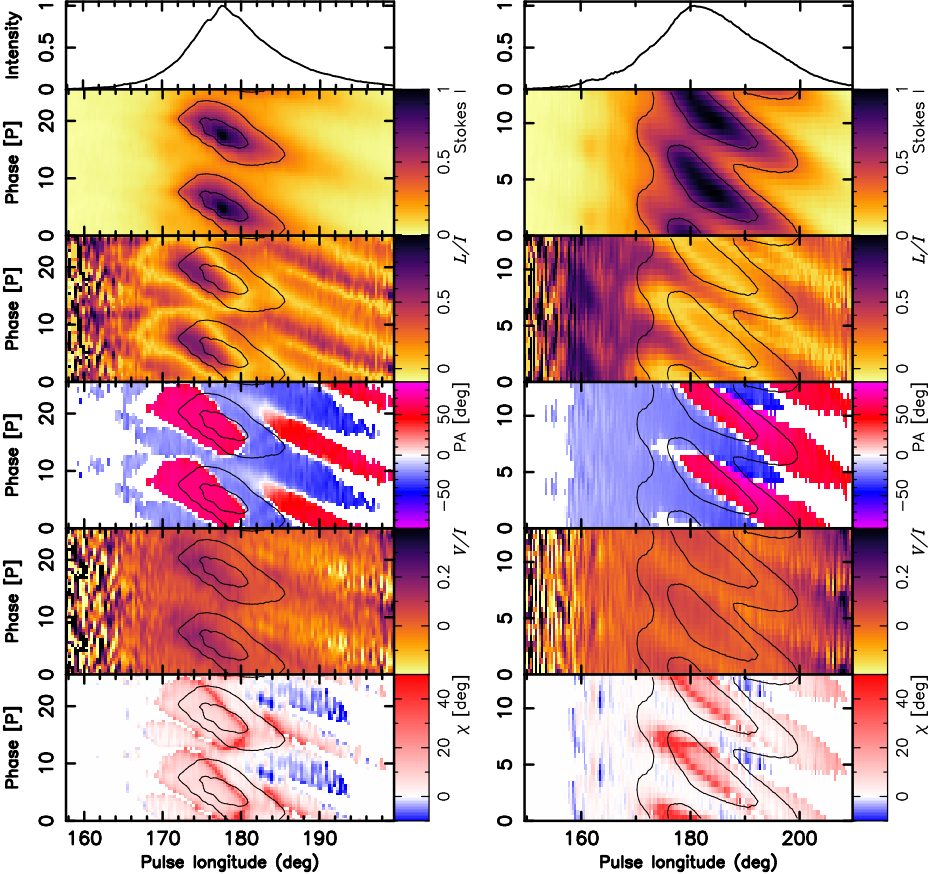
\includegraphics[width=1.0\textwidth]{Figures/B0031/observed_P3folds}
        \caption[The two P3-folded drift modes of PSR~B0031$-$07]{The two drift modes of PSR~B0031$-$07 folded at the period $P_3$. Mode A is shown in the left-hand column and mode B on the right. The total intensity driftbands are shown at the top, under the pulse profile. In descending order, the five colour plots are Stokes $I$, linear polarisation fraction $L/I$, PA, circular polarisation fraction $V/I$, and ellipticity angle $\chi$. The $P_3$ cycle is plotted twice for clarity, and the total intensity driftband is shown by the contour plots in the lower four plots of each mode. Figure recreated with permission from \citet{IWJ+2020}.}
        \label{fig: B0031 - observed P3folds}
    \end{center}
\end{figure}

The $P_3$-folds of both drift modes are shown in Fig.~\ref{fig: B0031 - observed P3folds} and reveal that the A (left-hand panels) and B (right-hand panels) drift patterns of PSR~B0031$-$07 are very different. In total intensity (top panels) pattern A exhibits bright, concentrated emission in the leading half of the driftbands followed by a much fainter and gradually dimming tail, whereas pattern B has a wider and somewhat more symmetrical pattern. Both seem to show a bend in the driftband at around pulse longitude $\phi = 185\degr$, after which the band becomes more shallow. There is also evidence in pattern B for another small patch of modulated emission preceding the main driftband at pulse longitude $162\degr$, which is not present in pattern A. Even more complex are the position angle patterns (fourth row of panels in Fig.~\ref{fig: B0031 - observed P3folds}). For mode B only the trailing half of the profile shows periodic changes in PA, such that the OPM with a positive PA (represented by the red colouring) roughly traces the Stokes $I$ driftbands (indicated by the contours). This association of one OPM with the total intensity pattern resembles the behaviour of PSR~B0809+74 \citep{RRS+2002}. In mode A also the leading half of the pulse shows periodic modulation of the dominating OPM. For the leading half of the profile the OPM with a positive PA is mostly associated with the driftbands as seen in total intensity, while at $\phi \sim 180\degr$ the two OPMs seem to abruptly switch.

PSR~B0031$-$07 is not unique in showing OPM variability associated with drifting subpulses: other than PSR~B0809+74 \citep{ESxx2004,RRL+2006} periodic OPM switches have also been identified in PSR~B0320+39 and B0818$-$13 \citep{ESxx2004}, and PSR~B1237+25 \citep{RRxx2003}. In these pulsars the Stokes $I$ driftbands are dominated by one OPM with the other OPM occurring in between, whereas for drift mode A of PSR~B0031$-$07, the OPMs appear to switch {\it within} the Stokes $I$ driftband in the pulse longitude direction. This switching is problematic in the sense that it means that these observations cannot be explained by a static pattern of OPMs circulating the magnetic axis, the picture used to explain the observations of PSR~B0809+74. The aim of this work is to see if the polarised subpulse pattern of PSR~B0031$-$07 can be explained within the framework of the carousel model. The possibility that magnetospheric propagation effects are responsible for the asymmetric pattern observed in the PA $P_3$-fold is explored. Although asymmetric refraction cannot be ruled out, it is hard to model mathematically without any specific model that predicts the functional shape of refraction throughout the magnetosphere. A simpler model with many fewer degrees of freedom would be to consider that the two OPMs remain coupled during propagation through the magnetosphere \citep[e.g.][]{Pxxx2001}. In this context coupling means that power can be exchanged between the two modes; in addition, the OPMs may be attenuated, reducing the overall intensity. I suggest that the asymmetries observed arise from these longitude-dependent processes. It will be demonstrated that these processes cannot be uniquely constrained. Nevertheless, it will be found that solutions do exist that describe the observations in terms of a static, circulating pattern of sub-beams in line with the prediction of a carousel model.

The following sections will explain how the observed polarised intensity is separated into the intensity of two OPMs. The cartographic transforms of \citet{DRxx2001} are discussed along with the symmetry predicted by the carousel model. The cartographic transform cannot be used directly to map the circulating system of polarised sub-beams, as the magnetospheric distortions need to be considered -- the mathematical description used to quantify these distortions will be defined, as well as how they can be used to show that a static circulating pattern of polarised sub-beams can explain the asymmetric pattern of PA in both drift modes of PSR~B0031$-$07.



%%%%%%%%%%%%%%%%%%%%%%%%%%%%%%%%%%%%%%%%%%%%%%%%%%%%%%%%%%%%%%%%%%%%%%%%%%%%%%%%%%%%%%%%%%%%%%%%%
%%%%%%%%%%%%%%%%%%%%%%%%%%%%%%%%%%%%%%%%%%%%%%%%%%%%%%%%%%%%%%%%%%%%%%%%%%%%%%%%%%%%%%%%%%%%%%%%%




\section{Methods}
\label{sec: B0031 - methods}

\subsection{Magnetospheric distortions}
\label{sec: B0031 - methods - magnetospheric distortions}

It is known \citep[e.g.][]{ABxx1986,BAxx1986,Pxxx2000} that refraction can cause a spatial separation of the two OPMs, which originate from a common source. This spatial separation has been suggested as the reason for the presence of OPM transitions (e.g. \citealt{ESLx2003,ESxx2004}). Refraction is due to plasma density gradients in the magnetosphere. This plasma density is believed to have minima at both the magnetic pole and the boundary of the open-field-line region \citep[e.g.][]{LPxx1998}, and this was used by \citet{PLxx2000} to demonstrate how emission produced relatively close to the magnetic axis could be refracted inwards to the other side of the magnetic axis, whilst emission further out is refracted even further outwards. This pole crossing means that an observer may simultaneously receive emission which originated from either side of the magnetic axis. This effect can lead to the appearance of nested cones from a single carousel. In an axisymmetric plasma distribution, any refraction occurs entirely in the plane of the magnetic field lines. If the carousel consists of an odd number of sub-beams, then emission from a sub-beam that is refracted (O-mode) across the pole ought to be out of phase relative to the emission of the non-refracted (X-mode) sub-beam component. When refractive delays or retardation effects are considered \citep{ESLx2003}, the sub-beams might not appear exactly out of phase. Larger azimuthal offsets could be caused by symmetry-breaking by magnetospheric rotation, or a non-axisymmetric plasma distribution \citep{BCWx1991, PLxx2000}. This is potentially a good description for what has been observed for PSR~B0809+74 \citep{RRL+2006}.

In mode A of PSR~B0031$-$07, the position angle (PA) of linear polarisation undergoes an OPM transition \textit{within} a given total intensity driftband such that the Stokes $I$ driftband is associated with different OPMs at different pulse longitudes (see Fig.~\ref{fig: B0031 - observed P3folds}). This change implies that the perceived polarisation properties of a given sub-beam have changed as it circulates, so that the emission from one OPM dominates at later longitudes whilst the other becomes stronger as the sub-beam drifts to earlier longitudes. This observation, as shown in the $P_3$-fold, is reproducible over long timescales. This suggests that a propagation effect is responsible. The required asymmetry with rotational phase of the pulsar is potentially caused by anisotropies in the magnetosphere at altitudes much higher, and over larger scales, than the emission region. Although refraction could play a role in causing the observed asymmetries, it is hard to model mathematically with a small number of parameters without any specific model to predict the functional shape of the refraction throughout the magnetosphere. In the absence of such a refraction model it would be impossible to construct the underlying, undistorted map of how the sub-beam structure of the carousel appeared before being affected in this way.


A much more tractable, and arguably more intuitive alternative model for longitude-dependent asymmetry is coupling of the OPMs in such a way that power can be transferred between them as they travel, as illustrated in Fig.~\ref{fig: B0031 - coupling schematic}.
\begin{figure}
    \begin{center}
        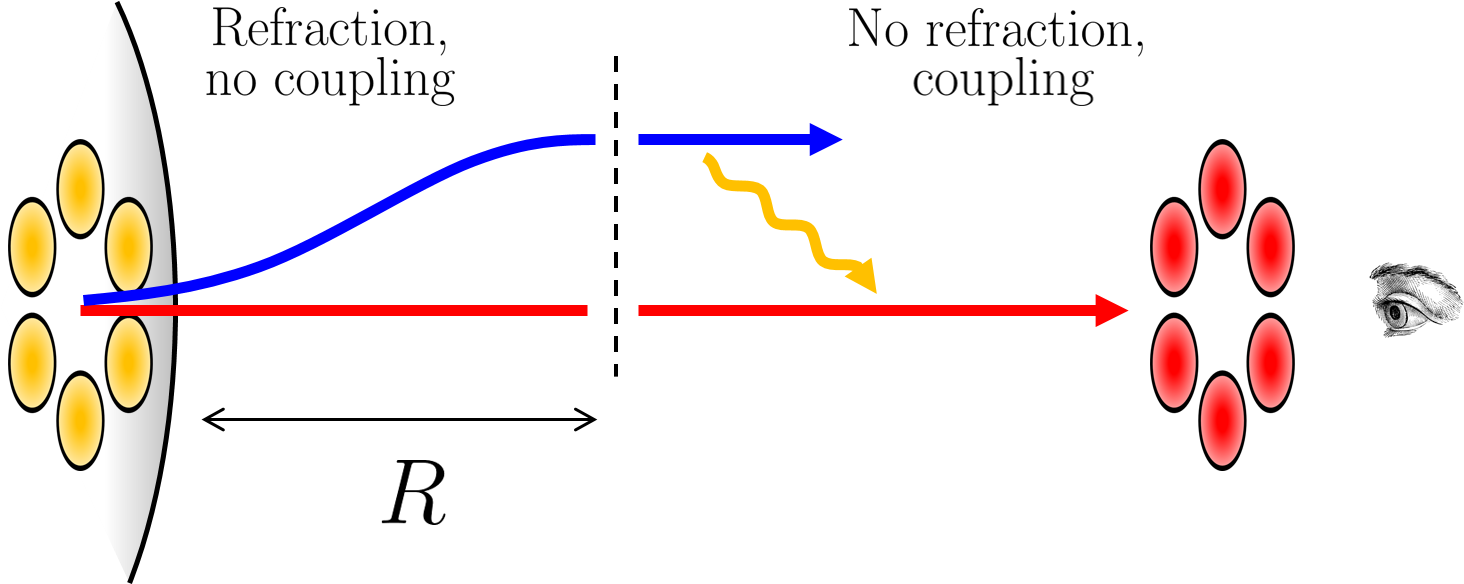
\includegraphics[width=0.7\textwidth]{Figures/B0031/coupling_schematic2}
        \caption[Schematic view of propagation of two OPMs through the magnetosphere]{A schematic representation of how refraction and mode coupling may occur in the pulsar magnetosphere. Two OPMs are generated at a common source, and propagate upwards. Below some radius $R$ refraction is the dominant effect, with the O-mode (blue) being refracted whilst the X-mode (red) travels freely. Above the limiting radius, refraction is no longer significant, whilst coupling becomes dominant. Power is allowed to be transferred between the two OPMs, and an observer sees the PA of the dominant OPM.}
        \label{fig: B0031 - coupling schematic}
    \end{center}
\end{figure}
Below some radius $R$, the propagation of the two OPMs is refraction-dominated: they originate from a common source, but the OPM identified with the O-mode is subject to refraction (blue in the figure), whereas the X-mode (red) is not \citep{ABxx1986}. The modes are not coupled in this region. At altitudes greater than $R$ refraction no longer plays an important role and coupling of the two modes becomes a strong effect. Any offset of the emission patterns due to refraction becomes `baked in', and the only further changes to the OPMs are due to the transfer of power between them and attenuation.
The idea of mode coupling is not new. \citet{Pxxx2000} suggested that refraction dominates only at low altitudes where the plasma density is sufficiently high. As the OPMs propagate outwards they enter a region where power may be transferred between the O- and X-modes. This conversion happens up to a certain height, after which the rays propagate independently again (unaffected by coupling or refraction). This model is discussed further in Sec.~\ref{sec: B0031 - discuss - general discusison}.
The assumption made in this work is that the observed asymmetry of PSR~B0031$-$07 is dominated by what happens above $R$. In that case there is a rotationally symmetric sub-beam structure produced by the carousel, possibly distorted (symmetrically) by refraction. The aim of this chapter is to deduce this maybe distorted, but overall axisymmetric, sub-beam structure from the observations.

This intrinsic beam structure circulates and would produce symmetrical driftbands and profile shapes. However, the modes are permitted to couple in a way which allows the modes to be mixed and attenuated above $R$. This transformation can be expressed by the simple matrix equation,
\begin{equation}
\label{eq: definition of the mixing matrix}
    \mathbf{O} = \begin{pmatrix} O_1\\O_2 \end{pmatrix} = \begin{pmatrix} M_{11} & M_{12}\\M_{21} & M_{22} \end{pmatrix} \begin{pmatrix} I_1\\I_2 \end{pmatrix} = \mathbf{MI},
\end{equation}
where $O_1$ and $O_2$ are the intensities of the observed OPMs (at a given pulse longitude and pulse number), $I_1$ and $I_2$ are the intensities of the `intrinsic' OPMs (i.e. before being affected by mode coupling), and $\mathbf{M}$ is the `mixing matrix' that parametrises the coupling and attenuation of the OPMs due to propagation through the magnetosphere. Absorption effects have been cited as the cause of asymmetric profiles \citep[e.g.][]{Rxxx1983b}, and this effect would correspond to the diagonal elements of $\mathbf{M}$. Mode coupling, including non-zero off-diagonal terms, can be seen as a generalisation of this concept.

In this model, the observed asymmetry is a consequence of the pulse longitude-dependence of the mixing matrix, which is otherwise taken to be independent of time during the modulation cycle. So there exists an intrinsic pattern of sub-beams (describing $I_1$ and $I_2$) that is static in the sense that their structure and polarisation properties are time-invariant apart from their circulation, and all asymmetry in the driftbands and profile is caused by mode coupling. The `intrinsic' driftbands (and hence carousels) to be recovered are the patterns of radiation seen after refraction has taken place, so some azimuthal and radial offset of the two OPM sub-beams can be expected. Under these assumptions, the mixing model should be able to reproduce the observed $P_3$-folds. Since the $P_3$-fold technique has effectively averaged many different beamlets, it is the average beam structure which will be described by the model, thereby ignoring additional stochastic variability. The symmetry of the circulating intrinsic intensity pattern can be exploited (at least up to some level) to isolate and remove the distortions caused by mode coupling -- to do this, we first separate the observed emission into the two observed OPMs, $O_1$ and $O_2$.

%%%%%%%%%%%%%%%%%%%%%%%%%%%%%%%%%%%%%%%%%%%%%%%%%%%%%%%%%%%%%%%%%%%%%%%%%%%%%%%%%%%%%%%%%%%%%%%%%
%%%%%%%%%%%%%%%%%%%%%%%%%%%%%%%%%%%%%%%%%%%%%%%%%%%%%%%%%%%%%%%%%%%%%%%%%%%%%%%%%%%%%%%%%%%%%%%%%






\subsection{Separating the OPMs}
\label{sec: B0031 - methods - mode separation}

To split the observed emission into the intensities of the two OPMs $O_1$ and $O_2$, the position angle (PA) and the linear polarisation fraction $L/I$ are taken into account at each point in the $P_3$-fold. Orthogonally polarised modes are in general thought to have PAs which differ by $90\degr$, and have equal but opposite ellipticities. They are therefore antipodal when represented on a Poincar\'e sphere. The expected signature of an OPM transition in a pulse profile is that when a PA jump occurs both the linear and circular polarisation fractions go to zero (complete depolarisation). However, for PSR~B0031$-$07 \citet{IWJ+2020} found that while the two modes are offset by $90\degr$ in PA, only one of the modes appears to have circular polarisation associated with it -- strictly speaking then the modes are non-orthogonal. The separation of non-orthogonal polarisation modes was explored by \citet{Mxxx2003} in the context of OPMs that are non-orthogonal in PA, highlighting that separating non-orthogonal OPMs is not possible without making additional assumptions to break the arising degeneracies. Further discussion of non-orthogonal modes can be found in Sec.~\ref{sec: B0031 - discussion}

The method used to split the observed emission into $O_1$ and $O_2$ is similar to that of \citet{MSxx2000} except that the circularly polarised intensity component was not considered. This is justified because throughout the profile the circularly polarised fraction is much weaker than the linear polarisation, as shown in the third ($L/I$) and fifth ($V/I$) rows of Fig.~\ref{fig: B0031 - observed P3folds}. The OPMs are assumed to combine incoherently to explain the observed unpolarised component of the radiation. Incoherent mode addition can readily explain the sudden PA jumps, while for coherent mode addition the PA transitions may be expected to be much smoother. This is discussed further in Sec.~\ref{sec: B0031 - discussion}. In the process of separating the OPMs in the $P_3$-fold, the Stokes parameters are rotated by the observed PA at a given longitude in the pulse profile which has the effect of removing any systematic pulse longitude-dependence of the PA caused by the Rotating Vector Model or otherwise. This means that these effects do not have to be considered in further analysis.

\begin{figure}
    \begin{center}
        \includegraphics[width=\textwidth]{Figures/B0031/observed_OPMs}
        \caption[PSR~B0031$-$07's two drift modes split into two OPMs]{The separated observed OPMs of the two drift modes, with drift mode A on the left and mode B on the right. The upper panel shows the integrated profiles of each OPM, normalised to the peak of the stronger of the two, with OPM 1 shown by the solid line and OPM 2 by the dashed line. The colour plots show the observed driftbands, with OPM 1 above and OPM 2 below. The mean pulse longitude-dependent intensity has been subtracted from these $P_3$-folds.}
        \label{fig: B0031 - observed OPMs}
    \end{center}
\end{figure}

Figure.~\ref{fig: B0031 - observed OPMs} shows the intensity of the separated observed OPMs for each drift mode, which are referred to as OPM 1 and OPM 2 respectively (the order is arbitrary). These $P_3$-folds have had the mean intensity subtracted from each pulse longitude column, so they do not show the full intensity pattern but rather the variation about the mean. This highlights the modulation pattern which should be reproduced by a circulating pattern of beamlets, on top of any unmodulated background emission. As described in Sec.~\ref{sec: B0031 - methods - calculating intrinsic emission} and Appendix~\ref{app: matrix maths - accounting for unmodulated emission}, subtracting the mean has the advantage that unmodulated emission is properly taken into account in the fitting process used to constrain the mixing matrix. 

OPM 1 of mode A (upper left panel) has a small blob of emission at the leading edge of the driftband at around $172\degr$ which is not present at the trailing edge; instead the driftband has a smooth tail. Similarly, OPM 2 (lower left panel) has concentrated emission in the leading half, but after pulse longitude $185\degr$ this fades out slowly in an extended tail. Mode B, shown in the right-hand panels of Fig.~\ref{fig: B0031 - observed OPMs}, is more complex than mode A, and extends across a larger longitude range. In OPM 1 (upper right panel), the observed  $P_3$-fold has a chequerboard-like structure in the leading half (up to $\sim$180$\degr$) before settling into stable continuous driftbands in the trailing half. OPM 2 (lower right panel) has a similar stable pattern which only becomes visible around $170\degr$ but extends past $200\degr$. These asymmetries will be exploited to find the distortions which will be quantified with the mixing matrix introduced in Sec.~\ref{sec: B0031 - methods - magnetospheric distortions}. From the shape of the observed driftbands predictions can be made about the form the mixing matrix must take: for example, the chequerboard pattern of mode B, OPM 2 may arise from two intrinsic modes which have symmetrical diagonal driftbands, offset from each other in pulse number. Mode conversion can make different intrinsic modes dominate at different longitude intervals in an observed OPM, thereby giving rise to such a chequerboard pattern.

In contrast, where the two observed OPM  $P_3$-folds have a very similar pattern, then one of the intrinsic modes may largely be suppressed, while the other is partially converted to the other observed mode. Such a scenario could be close to what is observed for the trailing half of mode B (right-hand panels of Fig.~\ref{fig: B0031 - observed OPMs}) after $\sim$185$\degr$, where the two OPMs appear very similar. In the following we will first quantify the expected symmetry for a circulating system of sub-beams. Any deviations from this should be explained with pulse longitude-dependent mode mixing.





%%%%%%%%%%%%%%%%%%%%%%%%%%%%%%%%%%%%%%%%%%%%%%%%%%%%%%%%%%%%%%%%%%%%%%%%%%%%%%%%%%%%%%%%%%%%%%%%%
%%%%%%%%%%%%%%%%%%%%%%%%%%%%%%%%%%%%%%%%%%%%%%%%%%%%%%%%%%%%%%%%%%%%%%%%%%%%%%%%%%%%%%%%%%%%%%%%%





\subsection{Carousel geometry}
\label{sec: B0031 - methods - carousel geometry}

During the rotation of the star, the orientation of the magnetic axis changes relative to the observer's line of sight (LOS). \citet{DRxx2001} defined a cartographic transform that maps the emission as recorded in a time series (i.e. a pulse stack and by extension a $P_3$-fold) onto a beam pattern relative to the magnetic axis. This allows an image of the radiation pattern to be constructed in a frame co-rotating with the carousel. The transform is defined by four parameters: the magnetic inclination angle, $\alpha$; the impact parameter of the LOS with respect to the magnetic axis, $\beta$; the period it takes for the carousel to complete one full circulation, $P_4$; and the pulse longitude corresponding to the fiducial plane, $\phi_\mathrm{fid}$. The fiducial plane is the plane in which the pulsar's magnetic and rotation axes lie. For an unaliased drifting subpulse pattern, the circulation period $P_4 \equiv NP_3$, where $P_3$ is the repetition period of the pattern in the pulse stack and $N$ is the number of sub-beams in the carousel. The transform used in this work is defined (Eqs.~\eqref{eq: cartographic transform - R}--\eqref{eq: cartographic transform - theta_rot}) and discussed in Appendix~\ref{app: geometry derivations}. This work extends the transform to include aliasing effects, which is discussed there too.

\begin{figure} [t]
	\begin{center}
	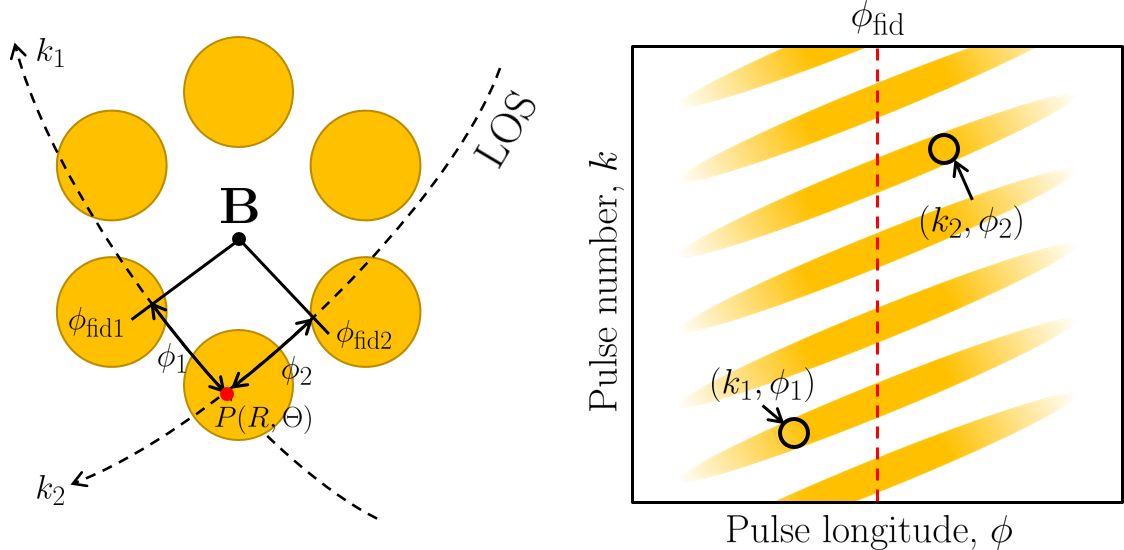
\includegraphics[width=0.9\textwidth]{Figures/B0031/opposite_points2}
	\caption[The predicted symmetry in driftbands arising from a circulating carousel]{An illustration of the argument that a carousel of sub-beams which remain unchanged during their circulation should produce `symmetric' pulse stacks such that two locations in the pulse stack have identical emission properties. LEFT: the carousel as viewed in a corotating frame. In this frame the line of sight appears to circulate, as is indicated for two stellar rotations $k_1$ and $k_2$. $\phi_\mathrm{fid 1,2}$ represents the location of the fiducial plane at each time. RIGHT: the pulse stack produced by such a carousel. The point $P$ intercepts the LOS at $k_1$ and $\phi_1$, and then the later at $k_2$ and $\phi_2$, so appearing in the pulse stack twice during a carousel rotation.}
    \label{fig: B0031 - symmetry}
    \end{center}
\end{figure}


As the carousel rotates, a given sub-beam will cross the observer's LOS twice, giving rise to an expected symmetry of the emission properties at two points on either side of the fiducial plane (see Fig.~\ref{fig: B0031 - symmetry}). In the left-hand panel a location in the carousel $(R, \Theta)$ -- labelled $P$ -- is intercepted by a LOS during the rotation number $k_1$ of the star at a longitude $\phi_1$. As the carousel circulates around the magnetic axis $(\vec{B})$, the point $P$ intercepts the LOS again at a later time (rotation $k_2$), this time at a different longitude $\phi_2$. This figure is drawn in a frame corotating with the carousel, so the carousel appears stationary while it is the LOS that moves. If the structure and intensity of the sub-beams do not change with time, the emission should be identical at points $(k_1,\ \phi_1)$ and $(k_2,\ \phi_2)$ in the pulse stack, shown on the right-hand side of Figure \ref{fig: B0031 - symmetry}. In folding the pulse stack at its modulation period $P_3$, the `average' driftband shape is found, meaning that the matching pair of points would be found in the same driftband. These points can be identified using the cartographic transform and methods explained in Appendix~\ref{app: geometry derivations - P3 fold - matching points}.

It should be noted that the transform used in this work, and the subsequent mathematics behind the argued symmetry of the drifting emission, is based on the assumption that the circulating carousel is perfectly circular. Elliptical carousels were proposed as an explanation for `bi-drifting' pulsars, where the subpulses move in opposite directions in different parts of the profile \citep{QLZ+2004, Wxxx2016, WWxx2017, SLWM2020}. This model still has an intrinsic symmetry, however it has more degrees of freedom and is significantly harder to describe mathematically. Therefore, in this work only simple, circular carousels are considered.





%%%%%%%%%%%%%%%%%%%%%%%%%%%%%%%%%%%%%%%%%%%%%%%%%%%%%%%%%%%%%%%%%%%%%%%%%%%%%%%%%%%%%%%%%%%%%%%%%
%%%%%%%%%%%%%%%%%%%%%%%%%%%%%%%%%%%%%%%%%%%%%%%%%%%%%%%%%%%%%%%%%%%%%%%%%%%%%%%%%%%%%%%%%%%%%%%%%






\subsection{Determining the intrinsic carousel emission}
\label{sec: B0031 - methods - calculating intrinsic emission}

As explained in Sec.~\ref{sec: B0031 - methods - carousel geometry}, the $P_3$-fold should obey an intrinsic symmetry with respect to the fiducial plane such that pairs of corresponding points can be identified in the $P_3$-fold (one in the leading half of the pulse and one in the trailing half). These pairs of points should intrinsically have the same (polarised) intensity. However, under the action of the mixing matrix (Eq.~\eqref{eq: definition of the mixing matrix}) differences can arise. To allow the polarisation to be intrinsically identical for the two points, Eq.~\eqref{eq: definition of the mixing matrix} can be used to link the two observed locations. This gives
\begin{equation}
    \label{eq: matching leading and trailing observed OPMs}
    \mathbf{O}^l = \mathbf{M}^l(\mathbf{M}^t)^{-1}\mathbf{O}^t \equiv \mathbf{A O}^t,
\end{equation}
where the superscripts $l$ and $t$ denote two corresponding points in the leading and trailing halves of the $P_3$-fold respectively. The `asymmetry matrix' $\mathbf{A}$ is defined such that
\begin{equation}
    \label{eq: definition of the asymmetry matrix}
    \mathbf{A}=\begin{pmatrix}A_{11} & A_{12}\\A_{21} & A_{22} \end{pmatrix}\equiv\mathbf{O}^l(\mathbf{O}^t)^{-1} = \mathbf{M}^l(\mathbf{M}^t)^{-1}.
\end{equation}
This equation can be defined for each combination of corresponding pulse longitudes, and each combination of corresponding phases during the $P_3$ cycle (where the phase corresponds to the vertical axes of Figs.~\ref{fig: B0031 - observed P3folds} and \ref{fig: B0031 - observed OPMs} for example).

Matrix $\mathbf{A}$ follows directly from the observed data and quantifies the observed asymmetry in the OPMs in the two corresponding points in the $P_3$-fold. This measure of asymmetry constrains a range of degenerate matrices $\mathbf{M}$ describing the propagation effects, and therefore implies that the condition for the intrinsic radiation pattern to be symmetrical is not enough to find unique solutions for the mixing matrix. All degenerate individual solutions  of $\mathbf{M}$ can mathematically explain the observed radiation equally well, as discussed further later in this subsection.

In Sec.~\ref{sec: B0031 - methods -  magnetospheric distortions} the assumption was made that the mixing matrix only depends on pulse longitude, and is otherwise independent of time. This means that the matrix $\mathbf{A}$, which can be evaluated using Eq.~\eqref{eq: definition of the asymmetry matrix} at different phases during the modulation cycle for a given pair of pulse longitudes, would ideally be identical. In reality, noise in the data causes (insignificant) differences. In addition, there will be systematic errors involved resulting from the observed emission being incompatible with the geometrical assumptions made. Fitting methods can be used to define an optimal $\mathbf{A}$ averaged over the modulation cycle.

Eq.~\eqref{eq: matching leading and trailing observed OPMs} can be written out as a set of equations for each $P_3$-fold bin $i$ during the modulation cycle and each of the two OPMs $j = \{1,2\}$,
\begin{equation}
    \label{eq: matched observed OPMs - simultaneous equations}
    O_{j,i}^l - A_{j1}O_{1,i}^t - A_{j2}O_{2,i}^t = 0.
\end{equation}
The fitting process results in the matrix $\mathbf{\hat{A}}$ which optimally applies throughout the modulation cycle, and which minimises
\begin{equation}
    \label{eq: chi-squared function for asymmetry matrix}
    \chi_j^2 = \sum_i{\frac{(O_{j,i}^l - \hat{A}_{j1}O_{1,i}^t - \hat{A}_{j2}O_{2,i}^t)^2}{\sigma_{O_j}^2 + \hat{A}_{j1}^2\sigma_{O_1}^2 + \hat{A}_{j2}^2\sigma_{O_2}^2 }},
\end{equation}
where the $\sigma^2$ terms are the variances\footnote{Here the noise in $O_1$ and $O_2$ are taken to be independent, random variables, which are moreover uncorrelated in different pulse longitude bins.} as determined in the off-pulse region of the corresponding OPMs. As Eq.~\eqref{eq: chi-squared function for asymmetry matrix} is non-linear due to the weight term (denominator), it should be solved using numerical methods to find the minimum. In practice, minimising Eq.~\ref{eq: chi-squared function for asymmetry matrix} does not lead to satisfactory results as often the minimum corresponds to a solution which looks noise-like with a $\chi^2 \simeq 1$. This corresponds to the situation where the mixing matrices are chosen such that the intrinsic polarisations have, effectively, most signal suppressed, leaving essentially only noise. An effective way to find physically more meaningful solutions is by minimising Eq.~\ref{eq: chi-squared function for asymmetry matrix} with the denominator set to 1 (an unweighted fit). This ensures that the observed polarisation signatures in the two corresponding longitudes at both sides of the fiducial plane can be matched via the mixing matrix, giving rise to a constrained underlying sub-beam pattern. A consequence of using the solution arising from the unweighted fit is that it is not necessarily optimum in terms of the weighted $\chi^2$. However, if the weighted $\chi^2$ for the solution found by solving the unweighted equation is still good, we know that a good solution exists. We will therefore be able to demonstrate that satisfactory solutions exist, which is the main aim of this work. Although Eq.~\eqref{eq: chi-squared function for asymmetry matrix} is solved without considering the weight term, all quoted $\chi^2$ values include it.

Since solving Eq.~\eqref{eq: chi-squared function for asymmetry matrix} without the weighting term is a linear problem, standard linear regression methods \citep[e.g.][]{NumericalRecipes} could be used. Furthermore, a physical constraint can be applied arising from the fact that intensities are nonnegative quantities. Therefore, all elements of $\mathbf{M}$ should be nonnegative $(M_{ij} \geq 0)$. This requirement translates to constraints upon $\mathbf{A}$ as derived in Appendix \ref{app: matrix maths - physical constraints}. Appendix \ref{app: matrix maths - posmatrix explanation} explains how a constraint on $\mathbf{A}$ can be used to constrain the range of possible solutions for the mixing matrix which are compatible with $\mathbf{A}$. In summary, a penalty is imposed on the $\chi^2$ should the initial solution from a standard linear regression prove `unphysical' -- overall, the mixing matrix is fitted using the downhill simplex algorithm \citep{NMxx1965} and is forced to only return physical matrices. Equation~\eqref{eq: chi-squared function for asymmetry matrix} defines the $\chi^2$ for a single pulse longitude bin only. To calculate the overall goodness-of-fit we sum the $\chi^2$ for each pulse longitude bin in the observed $P_3$-folds where there is a high signal-to-noise ratio (S/N). In the sum, pulse longitude bins for which the `opposite' bin also lies within the high S/N region are given double weight.

Eq.~\eqref{eq: matching leading and trailing observed OPMs} assumes that the observed emission can be described as an intrinsically symmetrical pattern modified only by the mixing matrix. However, there is also some form of (asymmetric) unmodulated background emission in the data which is not expected to share the same symmetry, since it is not caused by circulation. As explained more thoroughly in Appendix~\ref{app: matrix maths - accounting for unmodulated emission}, the effect of the unmodulated emission can be mitigated effectively by subtracting the mean intensities in the $P_3$-fold for each pulse longitude as has been done in Fig.~\ref{fig: B0031 - observed OPMs}.

The matrix $\mathbf{\hat{A}}$, and by extension the mixing matrix, parametrises the magnetospheric distortions that lead to the observed asymmetry. Once determined, it is possible to invert Eq.~\eqref{eq: definition of the mixing matrix} to reveal the intrinsically symmetrical pattern of polarised emission produced by the underlying carousel.







%%%%%%%%%%%%%%%%%%%%%%%%%%%%%%%%%%%%%%%%%%%%%%%%%%%%%%%%%%%%%%%%%%%%%%%%%%%%%%%%%%%%%%%%%%%%%%%%%
%%%%%%%%%%%%%%%%%%%%%%%%%%%%%%%%%%%%%%%%%%%%%%%%%%%%%%%%%%%%%%%%%%%%%%%%%%%%%%%%%%%%%%%%%%%%%%%%%




\subsubsection{Degeneracies in the results}
\label{sec: B0031 - methods - calculating intrinsic emission - degeneracies}

A constrained asymmetry matrix $\mathbf{A}$ does not map to a unique form of the mixing matrix $\mathbf{M}$. There is a major degeneracy which follows from Eq.~\eqref{eq: definition of the asymmetry matrix}: the asymmetry matrix $\mathbf{A}$ is a combination of the mixing matrix for two different pulse longitudes at each side of the fiducial plane, $\mathbf{M}^l$ and $\mathbf{M}^t$ respectively. Any values for the elements of these two mixing matrices are equally valid, as long as they satisfy Eq.~\eqref{eq: definition of the asymmetry matrix} (and are considered `physical' as detailed in Appendix \ref{app: matrix maths - physical constraints}). 

A consequence of this degeneracy is that an arbitrary scaling (by a positive number) can be applied to each corresponding pair of pulse longitudes. This means that the intrinsic emission could be arbitrarily bright, as long as it gets suitably attenuated by the mixing matrix. In order to mitigate this, the mixing matrices are normalised, such that the quadrature sum of the determinants\footnote{The determinant is involved in calculating $\mathbf{M}^{-1}$ which transforms the observed polarisation to the intrinsic polarisations.} of $\mathbf{M}^l$ and $\mathbf{M}^t$ is one. The result of normalising the mixing matrices is a relatively smooth intrinsic sub-beam structure without wildly fluctuating intensities corresponding to different longitudes.

A further consequence of the degeneracy is that $I_1$ and $I_2$ can be swapped, which corresponds to a swap of the columns of $\mathbf{M}^l$ and $\mathbf{M}^t$. To ensure as smooth an underlying carousel structure as possible, we adopt the following procedure. Starting at the fiducial plane position of the profile we work our way outwards: solutions are obtained and it is determined on a longitude-bin-by-longitude-bin basis if swapping the intensity of $I_1$ and $I_2$ makes the result smoother -- this is achieved by comparing cross-correlations between the result for the previous more inner solutions with the swapped and unswapped results.







%%%%%%%%%%%%%%%%%%%%%%%%%%%%%%%%%%%%%%%%%%%%%%%%%%%%%%%%%%%%%%%%%%%%%%%%%%%%%%%%%%%%%%%%%%%%%%%%%
%%%%%%%%%%%%%%%%%%%%%%%%%%%%%%%%%%%%%%%%%%%%%%%%%%%%%%%%%%%%%%%%%%%%%%%%%%%%%%%%%%%%%%%%%%%%%%%%%









\subsection{Exploring parameter space}
\label{sec: B0031 - methods - parameter space}

Fitting the asymmetry matrix $\mathbf{A}$ requires matching pairs of pulse longitudes in the leading and trailing halves of the data, $\mathbf{O}^l$ and $\mathbf{O}^t$ respectively. Within these columns, which are equidistant from the fiducial plane position $\phi_\mathrm{fid}$, there are matching $P_3$ phases which are offset. These points have the same coordinates $R$ and $\Theta$ in the carousel frame, which correspond to the radial angular distance from the magnetic axis and azimuthal angle respectively. As explained in Sec.~\ref{sec: B0031 - methods - carousel geometry} (and in more detail in Appendix~\ref{app: geometry derivations - cartographic transforms - reverse transformation}), driftbands should be symmetrical about the fiducial plane, along contours of constant $\Theta$. The shape of the contours (and hence the phase of the corresponding points) is determined by knowledge of the geometry of the circulating beam pattern, specifically the parameters $\alpha$, $\beta$, and $P_4$. For a given set of these parameters, a fit can be performed for each pair of longitudes either side of the fiducial plane to determine the elements of $\mathbf{A}$, and the goodness of this fit (Eq.~\eqref{eq: chi-squared function for asymmetry matrix}) provides an indication of how symmetrical the points are: that is, how well can the observed intensity pattern in the $P_3$-fold be explained by a circulating beam pattern, which must produce symmetrical driftbands.

Because there are no assumption-free measurements or theoretical predictions of the required parameters, the parameter space was explored with a grid search. These parameters are $\phi_\mathrm{fid}$, $\alpha$, $\beta$, and $P_4$, however a slightly different (but mathematically equivalent) set of parameters were used to define the explored grid.

First of all, $P_4$ is related to $P_3$ (see Eq.~\ref{eq: geometry derivations - aliasing equation P3}). Hence, only discrete values of $P_4$ are allowed, which can be parametrised by the number of sub-beams in the carousel $N$ and the alias order $n$. For each parameter, four possibilities were explored (see Tab.~\ref{tab: atlas parameters}). The four values of both $N$ and $n$ includes two odd and two even numbers. The spacing of $N$ is such that the atlas covers a very low number up to around what is theorised by \citet{MBW+2019}. The fact that there are even and odd $n$ ensures that both inner and outer lines of sight are required -- an inner line of sight is where the LOS passes between the magnetic and rotation poles, and an outer line of sight is where the LOS passes between the magnetic pole and the equator. Apart from the lowest two orders of $n$ some higher orders were explored as well. However, from experimenting it was established that increasing the alias order further has little qualitative impact on the results.

For $\alpha$ four values were chosen, representing cases from a nearly aligned rotator to a fairly oblique rotator. The pulse profile of PSR~B0031$-$07 is wide, so it is unlikely to be close to orthogonal \citep[e.g.][]{SMS+2007}. Initially three values for $\phi_\mathrm{fid}$ were chosen. One of the choices for $\phi_\mathrm{fid}$ corresponds to $\phi_\mathrm{fid} = 182\degr$, which is slightly later than the peak of the total intensity profile. This is motivated by the observation that this is the approximate longitude at which the OPM transition occurs in the middle of the driftbands in mode A, as shown in the top right panel of Fig.~\ref{fig: B0031 - observed P3folds}. By placing the fiducial plane here, we force mixing to be responsible for as much of this asymmetry as possible. Two more longitudes were chosen to place the fiducial plane earlier or later to provide a contrast ($172\degr$ and $192\degr$). However, experiments over a sparse grid found that the early and late positions of the fiducial plane resulted in poor results, so these were not explored any further. A summary of the parameters we explore is shown in Tab.~\ref{tab: atlas parameters}. 
\begin{table}
    \centering
    \caption[Summary of the atlas geometry parameters]{A summary of the geometry parameters used in the atlas of results. Values labelled with a $\dagger$ were initially explored, but deemed unsatisfactory for further analysis}
    \label{tab: atlas parameters}
    \begin{tabular}{lc}
        \hline
        Parameter & Values  \\
        \hline
        $\alpha$ & $5\degr$, $15\degr$, $30\degr$, $60\degr$ \\
        $N$ & 5, 8, 11, 14 \\
        $n$ & 0, 1, 5, 10 \\
        $\phi_\mathrm{fid}$ & $^\dagger172\degr$, $182\degr$, $^\dagger192\degr$ 
    \end{tabular}
\end{table}

To make the grid search more efficient, the remaining parameter $\beta$ is not searched over. Instead it is fixed for given set of $\alpha$, $N$ and $n$ by making the predictable resulting gradient of the driftband (Eq.~\eqref{eq: driftband gradient} in Appendix~\ref{app: geometry derivations - P3 fold}) at $\phi_\mathrm{fid}$ match the actual driftband gradient. The driftband gradient is something which needs to be reproduced for the results to be considered `satisfactory'. For each choice of the other parameters, the driftband gradient was optimised by performing a grid search over a range of values with a step size of $0.1$~$P/\text{rad}$ (periods per radian; $1.7\times10^{-3}$~$P/\degr$ ). The assumed range is $-40$ to $-30$~$P/\text{rad}$ ($-0.70$ to $-0.52$~$P/\degr$) for mode A, and $-25$ to $-20$~$P/\text{rad}$ ($-0.44$ to $-0.35$~$P/\degr$) for mode B. The best gradient in this grid search was that which produced the lowest $\chi^2$ as explained in Sec.~\ref{sec: B0031 - methods - calculating intrinsic emission}.






%%%%%%%%%%%%%%%%%%%%%%%%%%%%%%%%%%%%%%%%%%%%%%%%%%%%%%%%%%%%%%%%%%%%%%%%%%%%%%%%%%%%%%%%%%%%%%%%%
%%%%%%%%%%%%%%%%%%%%%%%%%%%%%%%%%%%%%%%%%%%%%%%%%%%%%%%%%%%%%%%%%%%%%%%%%%%%%%%%%%%%%%%%%%%%%%%%%








\section{Application to \texorpdfstring{PSR~B0031$-$07}{PSR~B0031--07}}
\label{sec: B0031 - results}

As there is no \textit{a priori} information on how the carousel should appear, and it cannot be uniquely deduced from the methods applied here, we first apply a model using a set of parameters motivated by those reported in the literature. These results will be referred to as the `canonical model'. 

\subsection{The canonical model}
\label{sec: B0031 - results - literature}

For the number of sub-beams in the carousel, we take $N_A = 15$ for drift mode A and $N_B = 14$ for mode B. These values come from the work of \citet{MBW+2019} who investigated how aliasing coupled with a change in the number of sub-beams may explain the different $P_3$ values in PSR~B0031$-$07. Alongside the number of sub-beams, \citet{MBW+2019} also predict that both modes have an alias order $n = 1$, so first-order aliasing. The relationship between the alias order and number of sub-beams in this model are discussed further in Sec.~\ref{sec: B0031 - discussion}. There are no strong \textit{a priori} constraints related to where the fiducial plane lies, and we will only assume that it should lie somewhere within the bounds of the pulse profile. For the canonical model we make the choice to place the fiducial plane at $\phi_\mathrm{fid} = 182\degr$, which is slightly later than the peak of the total intensity profile of drift mode A. This is the approximate longitude at which the OPM transition occurs in the middle of the driftbands in mode A, as shown in Fig.~\ref{fig: B0031 - observed P3folds}. By placing the fiducial plane here, OPM mixing is forced to be responsible for as much of this asymmetry as possible, which is the primary reason to explore this methodology. The remaining not directly measurable parameters are $\alpha$ and $\beta$. \citet{SMS+2007} proposed that $\alpha \approx \beta$ for PSR~B0031$-$07, and that both lie in the range 2 to $4\degr$. We take $\alpha = 5\degr$ as a compromise between making $\alpha$ small, but not too small so as to make the canonical model an extreme geometry. For the model to be robust it should not rely on fine-tuned parameters. The value of $\beta$ is chosen to be consistent with the measured driftband gradients, as explained next. 

The driftband gradients used in the canonical model were estimated from the total intensity $P_3$-folds of mode A and mode B. For mode A, the gradient is observed to lie in the range $-40$ to $-30$~$P/\text{rad}$ ($-0.70$ to $-0.52$~$P/\degr$), and for mode B the range is $-25$ to $-20$~$P/\text{rad}$ ($-0.44$ to $-0.35$~$P/\degr$). To constrain $\beta$ in the canonical model parameter choice, four parameters ($N$, $n$, $\alpha$, and $\phi_\mathrm{fid}$) were fixed and the driftband gradient was permitted to vary within its range for mode B. The gradient which produced the best fit (i.e. the lowest reduced-$\chi^2$ as defined by Eq.~\ref{eq: chi-squared function for asymmetry matrix}) was found using a grid search, and this was $m_B = -24.5$~$P/\text{rad}$ ($-0.43$~$P/\degr$). This then defined $\beta = 7.4\degr$ via Eq.~\eqref{eq: geometry derivations - beta from gradient} which in turn defines the expected driftband gradient of mode A, $m_A = -49.2$~$P/\text{rad}$ ($-0.86$~$P/\degr$) via Eq.~\eqref{eq: driftband gradient} while keeping $\beta$ the same for both drift modes. This required gradient is steeper than the estimates, but not excessively so. This might lead to the parameters picked for the canonical model being sub-optimal, and gives one justification to explore a wider parameter range as is done for the atlas results that are discussed in Sec.~\ref{sec: B0031 - results - atlas}. The grid search was done for mode B, as it has more complex polarised subpulse structure (the chequerboard pattern in the leading half) and occupies a larger span of pulse longitudes compared to mode A. This means that it is likely to be more sensitive to the expected driftband shape, and so should take priority if a good fit is to be produced for both modes. A summary of the parameters that define the canonical model geometry is given in Tab.~\ref{tab: B0031 - literature parameters}.

\begin{table}
    \centering
    \caption[Parameters of the canonical model]{A summary of the parameters used in the canonical model geometry.}
    \label{tab: B0031 - literature parameters}
    \begin{tabular}{lc}
        \hline
        Parameter & Value \\
        \hline
        $\alpha$            & $5.0\degr$\\
        $m_B$               & $-24.5$~$P/\text{rad}$ ($-0.43$~$P/\degr$)\\
        $m_A$               & $-49.2$~$P/\text{rad}$ ($-0.86$~$P/\degr$)\\
        $\beta$             & $7.4\degr$\\
        $N_A$               & $15$\\
        $N_B$               & $14$\\
        $n_{A,B}$           & $1$\\
        $\phi_\mathrm{fid}$ & $182\degr$   
    \end{tabular}
\end{table}


\begin{landscape}
    \begin{figure}
        \begin{center}
            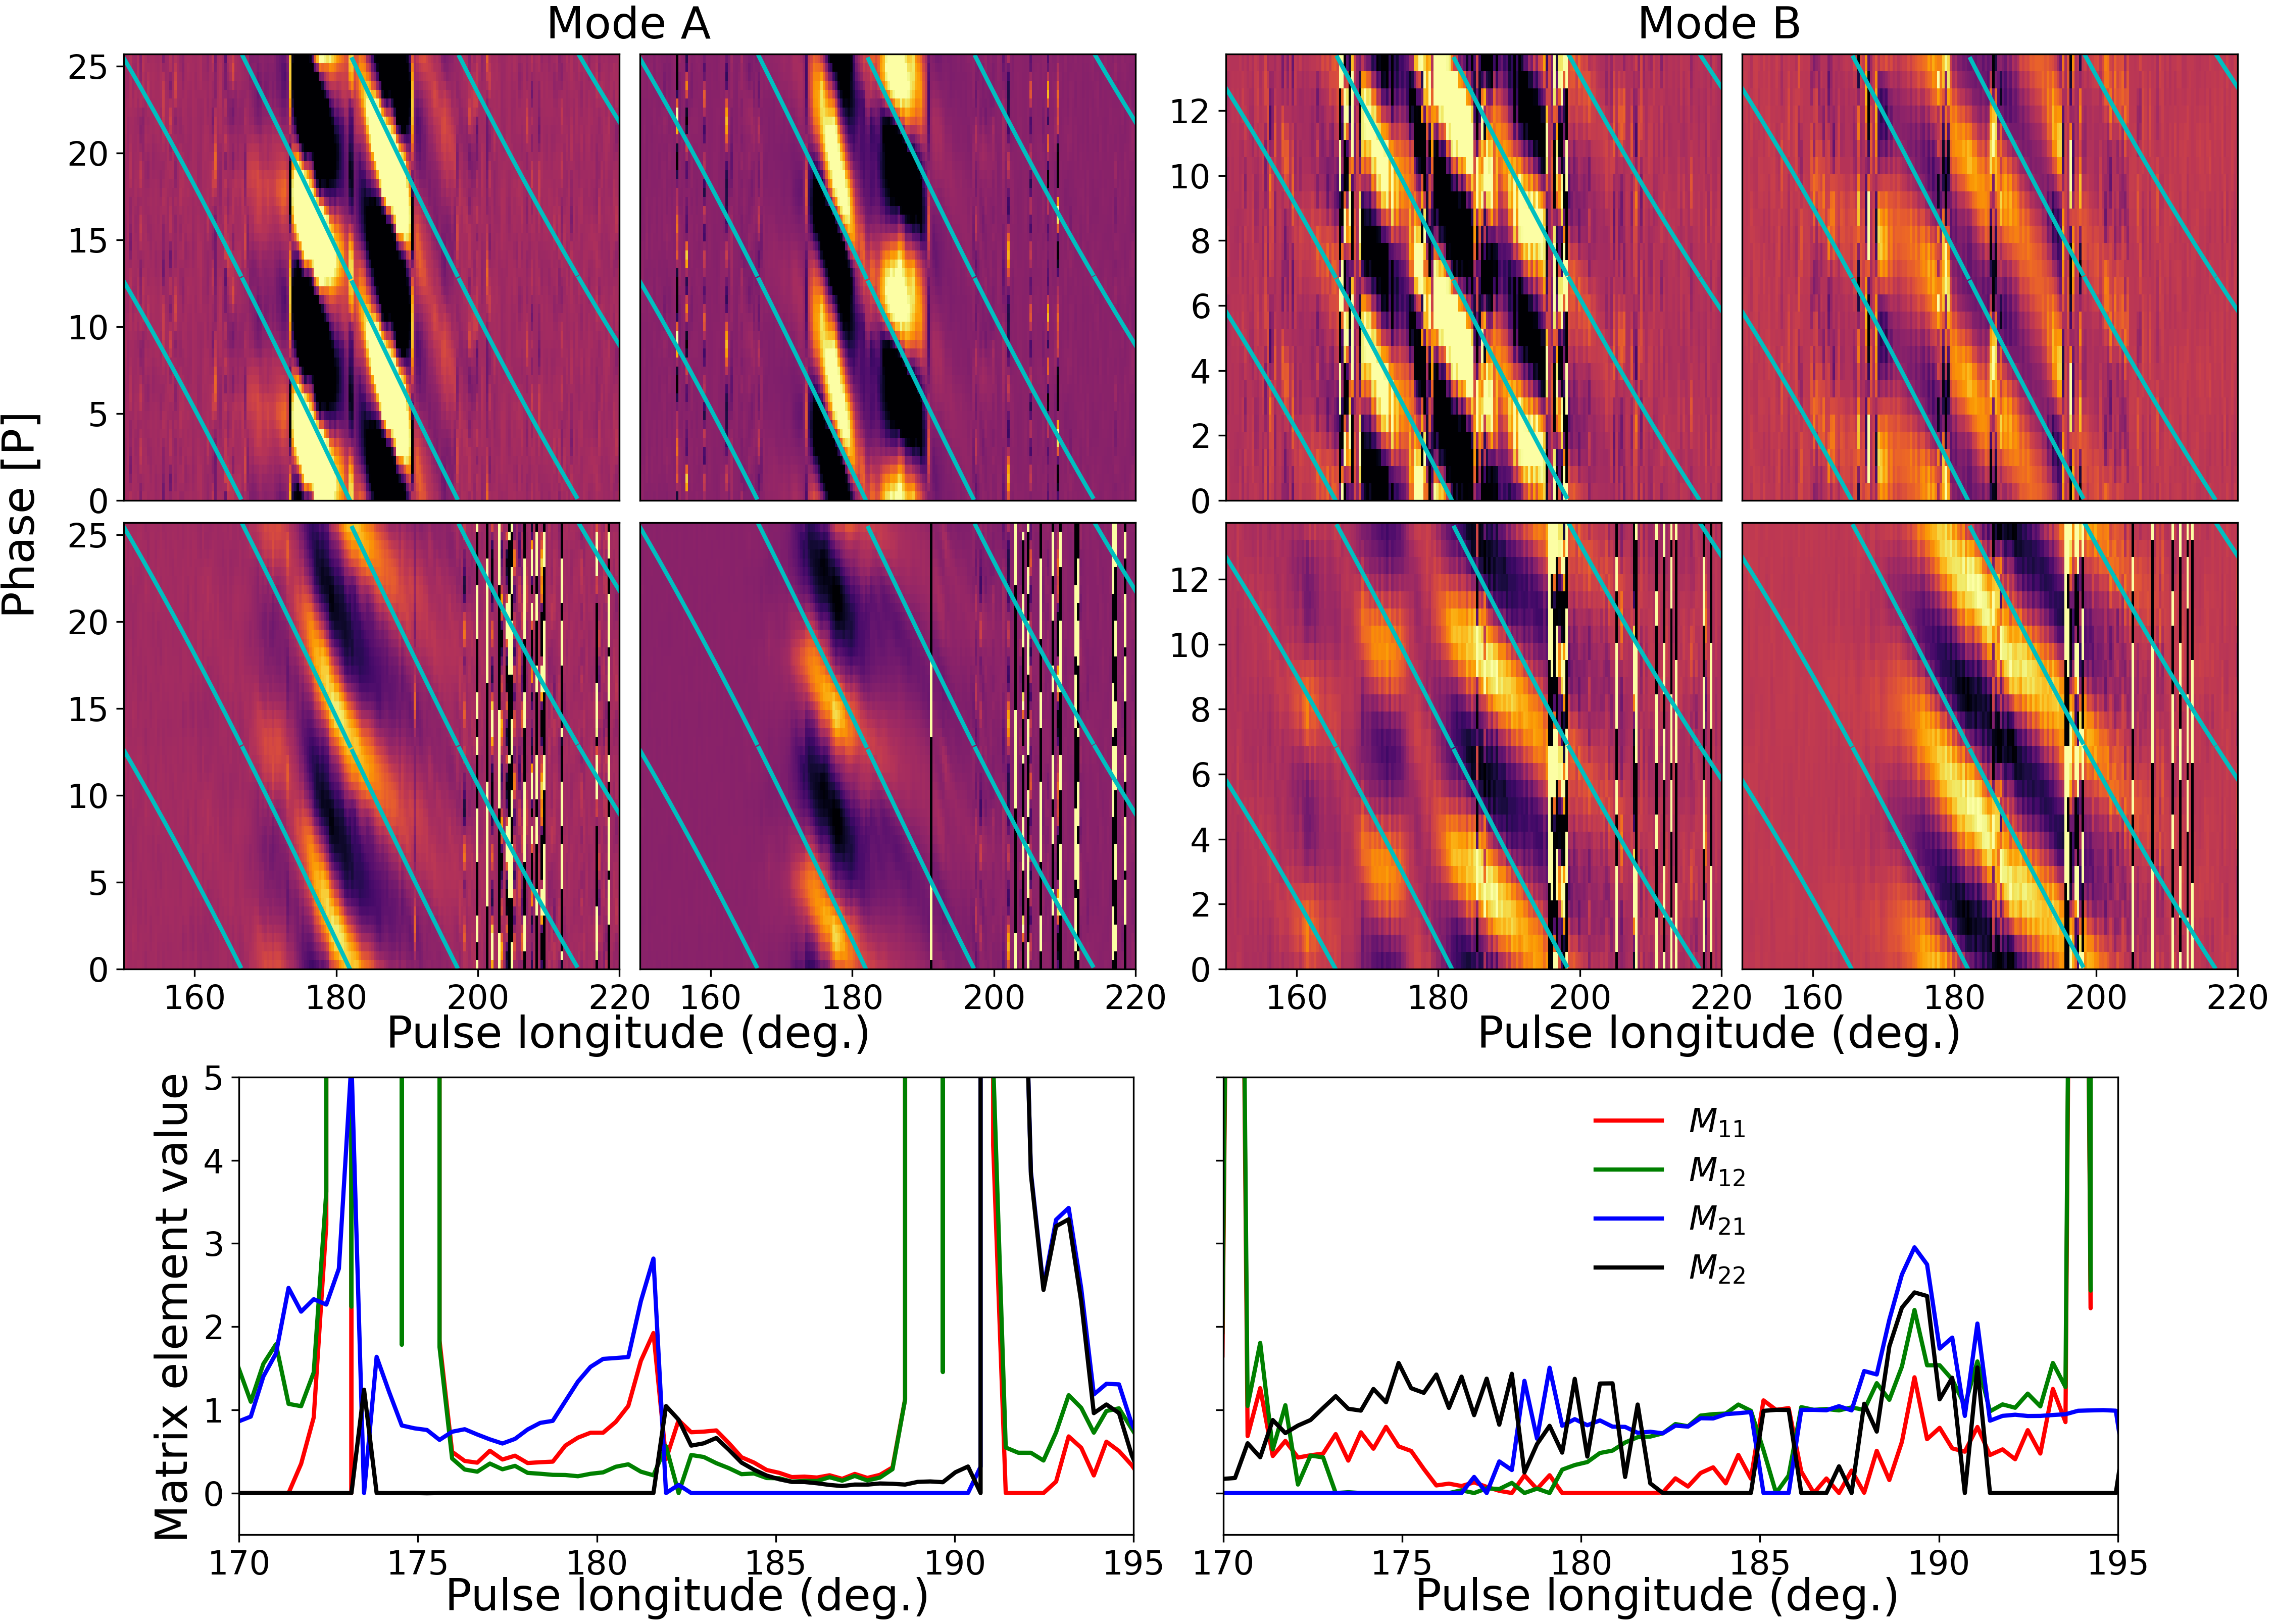
\includegraphics[height=0.66\textwidth]{Figures/B0031/canres_driftbands_2}
            \caption[Results for the canonical model]{The intrinsic and recreated observed driftbands found for the canonical model parameters for each drift mode, along with the associated mixing matrices. Mode A is plotted on the left, and mode B on the right. The upper row of the colour maps shows the intrinsic driftbands, with (arbitrarily labelled) OPM 1 on the left, and OPM 2 on the right. The cyan line shows the contours of constant $\Theta$. The lower colour map shows the recreated observations, which closely match the observed OPMs for each mode as shown in Fig.~\ref{fig: B0031 - observed OPMs}. In all panels the $P_3$ cycle is plotted twice for clarity. The lower line plots show the elements of the fitted mixing matrices as a function of pulse longitude. Where the matrix elements have extreme values as a result of poor fitting, these points have been `skipped' when plotting them, effectively being replaced by interpolated values in order to show the continuous structure. Similarly, the panels showing the driftbands have been clipped in order to show the structure that would otherwise be overwhelmed by the noisy pulse longitudes.}
            \label{fig: B0031 - canonical model driftbands and matrices}
        \end{center}
    \end{figure}
\end{landscape}
\begin{figure}
    \begin{center}
        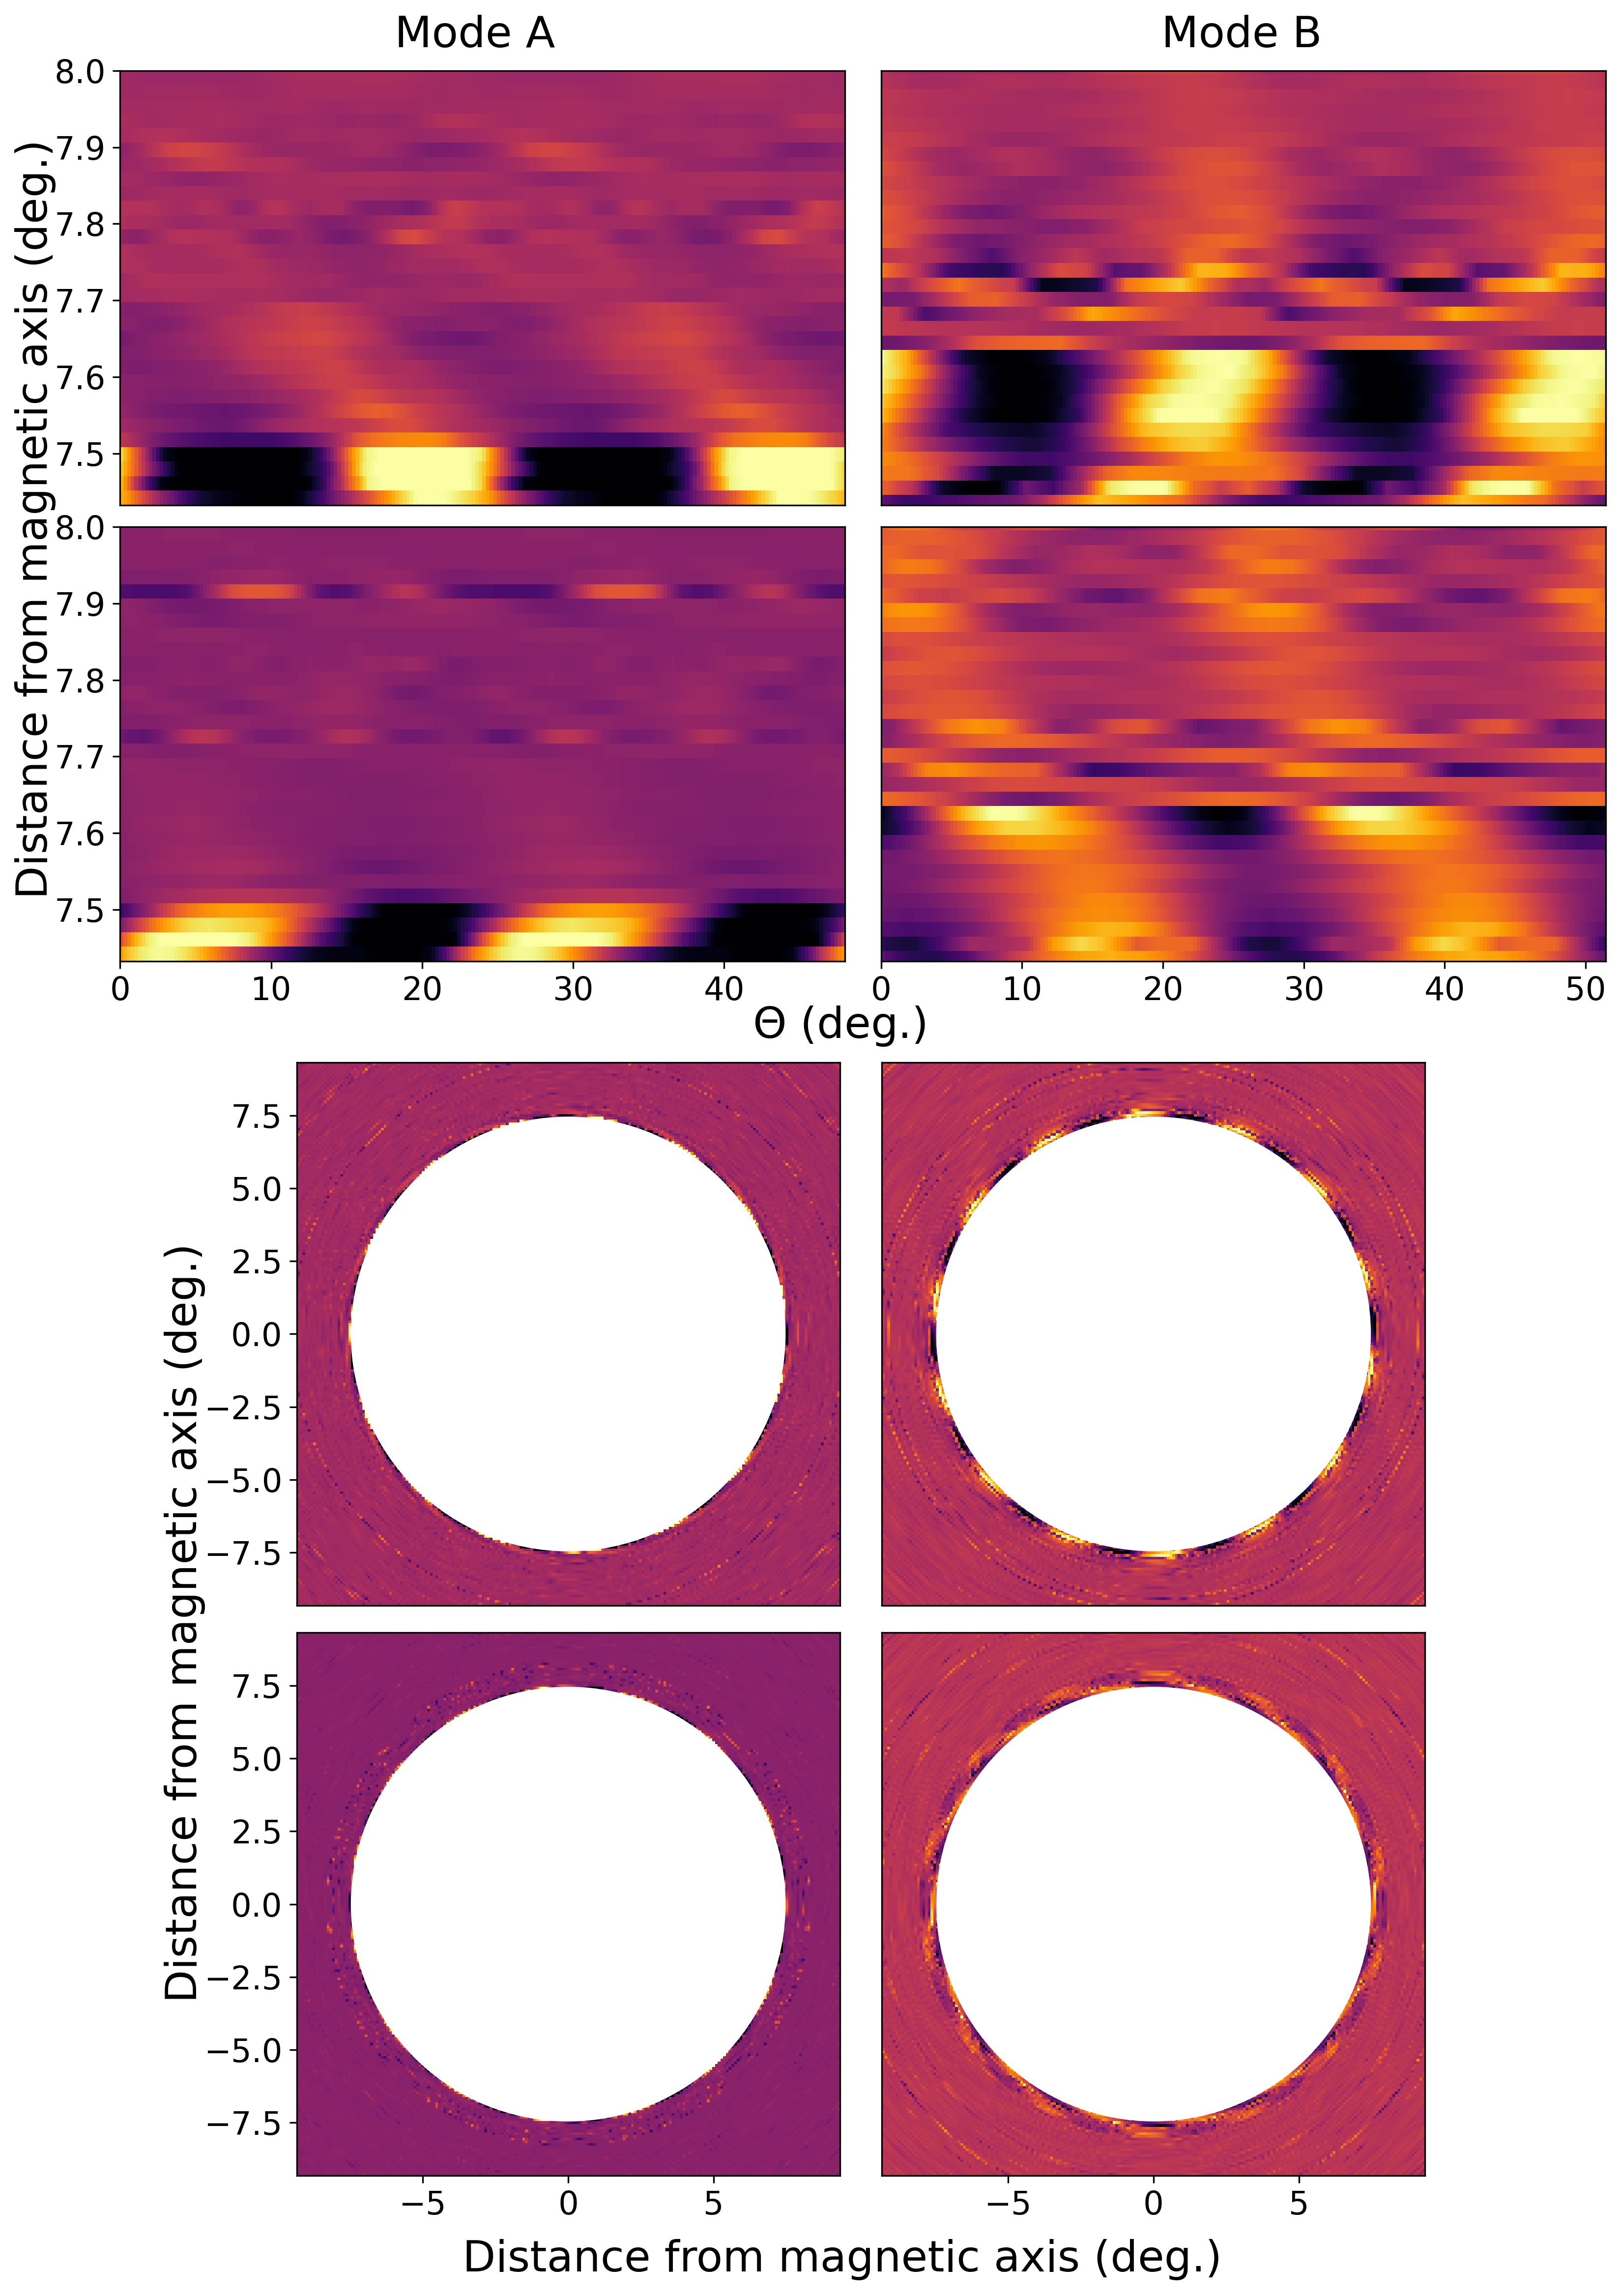
\includegraphics[width=0.8\textwidth]{Figures/B0031/canres_sparks_2}
        \caption[Sub-beams and carousels of the canonical model]{The intrinsic sub-beam structure and carousels of the two OPMs of each drift mode (mode A on the left, and mode B on the right). The upper four panels show a magnified view of the sub-beams in the carousel, plotted in polar coordinates that are treated as Cartesian for ease of illustration ($R$ on the $y$-axis, and $\Theta$ on the $x$-axis). Two sub-beams are shown for clarity. The upper row is OPM 1, and the lower row is OPM 2. The lower four panels show the full polar emission region for each OPM. Again, the upper row is OPM 1 and the lower is OPM 2. The white circle indicates the region where no emission can be observed because of the geometry of the LOS.}
        \label{fig: B0031 - canonical model sparks and carousels}
    \end{center}
\end{figure}

The results for the canonical parameter choice can be seen in Figs.~\ref{fig: B0031 - canonical model driftbands and matrices} and \ref{fig: B0031 - canonical model sparks and carousels}. Figure~\ref{fig: B0031 - canonical model driftbands and matrices} shows the intrinsic driftbands for each drift mode ($I_1$ and $I_2$) found by multiplying the observed OPMs (as seen in Fig.~\ref{fig: B0031 - observed OPMs}) by the inverse of the mixing matrix (Eq.~\eqref{eq: definition of the mixing matrix}). The cyan lines show the contours of constant $\Theta$ determined by the geometry parameters, and calculated using Eq.~\eqref{eq: geometry derivations - P3 phase definition}. For this set of parameters, the gradient of the expected driftband is close to being constant within the on-pulse window spanning $70\degr$. In mode A, OPM 1 has reasonably straight driftbands which closely match the model (cyan curve) whilst the driftbands of OPM 2 have a distinct V-shape -- this is indicative of the sub-beams in the carousel being swept azimuthally. In mode B, both bands trace the contour of constant $\Theta$. For both drift modes there are short intervals of pulse longitude where the driftbands appear discontinuous and noisy: these correspond to those longitudes where the fit was poor, resulting in a poorly constrained mixing matrix. The intrinsic OPM intensities are clipped to optimise the dynamic range of the figure for the regions of interest. The model attempts to find a symmetric intensity distribution in the $P_3$-fold. However, if the geometry parameters are sub-optimal, or if the assumptions made are somewhat oversimplified, there will be a residual asymmetry. To compensate for this, after creating the driftbands they are mirrored about the fiducial plane (along the contour of constant $\Theta$) and averaged. The results shown here are then symmetric. This therefore corresponds to the best-possible symmetric solution. The mixing matrix found is used to see if the observed emission can be reproduced satisfactorily from this symmetric pattern.

The second row of colour plots in Fig.~\ref{fig: B0031 - canonical model driftbands and matrices} show the reproduced observable OPMs using the intrinsic $P_3$-folds which were forced to be symmetric. Applying the mixing matrix to such $P_3$-folds highlights any asymmetries not captured by the model. These errors appear as the bright noise in the final panels, which lie mostly in the regions where little signal is available. The regions with a higher S/N are reproduced well for both modes, and show that the process has largely worked for the canonical model. It can be seen that the `recovered' $P_3$-folds closely match the original observed $P_3$-folds shown in Fig.~\ref{fig: B0031 - observed OPMs}. The chequerboard pattern in the leading half of mode B, OPM 1 has been successfully reproduced, as has the almost rectangular shape of mode A, OPM 2. The faint blob on the leading end of OPM 1 is also recovered well. 

The lower line plots in Fig.~\ref{fig: B0031 - canonical model driftbands and matrices} show the elements of the mixing matrix for drift mode A (left) and mode B (right) that is a result of the fitting at each longitude and after picking out a single solution via the procedure explained in Sec.~\ref{app: matrix maths - posmatrix explanation}. The four matrix elements are plotted in different colours: $M_{11}$ is shown in red, $M_{12}$ in green, $M_{21}$ in blue, and $M_{22}$ in black. For some longitudes, the fitting is poorly constrained because of noise in the data (most notably in the wings of the profile), resulting in erratic evolution of the elements as function of pulse longitude. Although there is some jagged variation in the values of the elements clearly visible in mode B, the matrices are generally smooth as a function of pulse longitude. This result is discussed further in Sec.~\ref{sec: B0031 - discuss - canonical model}.

In Fig.~\ref{fig: B0031 - canonical model sparks and carousels} a close-up view of individual sub-beams for each OPM and drift mode is shown in the top four plots. As in previous figures, mode A is shown in the left-hand panels and mode B in the right, while the upper panels show OPM 1 and the lower panels OPM 2. The sub-beams in these figures have been plotted in Cartesian coordinates, where the $x$-axis is the azimuthal angle in the carousel frame, $\Theta$, and the $y$-axis shows the distance from the magnetic axis, $R$. The minimum $R$-value corresponds to $R=\beta$, so the minimum $R$ probed by the LOS. In each panel of this figure two successive sub-beams are plotted for continuity. The sub-beams of OPM 1 of drift mode A are compact, and located close to the minimum radius but there is evidence of faint, swept-back emission at their outer edge. As predicted from the intrinsic OPM 2 driftband, the sub-beam for mode A is compact but strongly swept forwards. The sub-beams of both mode B OPMs are swept, and in opposite directions, although the sweep of OPM 2 is moderately more severe. Sweeping features could suggest that the canonical geometry is sub-optimal in explaining the observed polarisation, or that the model is somewhat oversimplified. Nevertheless, some sweep could be a real feature caused by refraction, as discussed in Sec.~\ref{sec: B0031 - discuss - atlas - atlas plots evaluation}. In both drift modes OPM 1 appears slightly more compact whereas OPM 2 is more elongated.

The lower four plots in Fig.~\ref{fig: B0031 - canonical model sparks and carousels} show a map of the carousel of sub-beams surrounding the magnetic axis. These illustrate how the carousel would appear to an observer looking down on the pulsar from above, and is the plane defined by the polar coordinates $R$ and $\Theta$ of the cartographic transform. As the structure circulates it is intersected by the observer's line of sight (LOS; not shown) as the star rotates, giving rise to the observed drifting subpulses. The sub-beams are distributed evenly in the azimuthal direction and are identical, a consequence of them being derived from the $P_3$-fold, thereby representing the average sub-beam morphology. There is a gap in the centre of the image for $R<\beta$ where there is no information as the LOS never samples this area. The fact that the sub-beams in both OPMs of both drift modes appear to be very thin in the radial direction whilst elongated in the azimuthal direction may indicate that the LOS only intersects the very edge of the sub-beam. The sub-beams may be larger and more symmetrical structures, with the majority of their emission occurring closer towards the magnetic axis and out of view of the observer.

The goodness-of-fit for the canonical set of parameters was $\chi^2_R = 6.6$ for mode A, and $\chi^2_R = 2.1$ for mode B. Although this indicates the observed emission cannot be fully explained by the model, it has performed very well in reproducing much of the complex behaviour, given the simplifying assumptions made. It also demonstrates the robustness of the model. It does not require fine-tuning to reproduce the data, as most parameters were not optimised to produce this canonical model.






%%%%%%%%%%%%%%%%%%%%%%%%%%%%%%%%%%%%%%%%%%%%%%%%%%%%%%%%%%%%%%%%%%%%%%%%%%%%%%%%%%%%%%%%%%%%%%%%%
%%%%%%%%%%%%%%%%%%%%%%%%%%%%%%%%%%%%%%%%%%%%%%%%%%%%%%%%%%%%%%%%%%%%%%%%%%%%%%%%%%%%%%%%%%%%%%%%%






\subsection{`Atlas' of parameters}
\label{sec: B0031 - results - atlas}

In order to test if the results for the canonical model can be considered robust (i.e. not strongly dependent on parameter choice), we created an atlas of results (as detailed in Sec.~\ref{sec: B0031 - methods - parameter space}) covering different values of each parameter. The full atlas covers a set of 64 different combinations of parameters for each of the two drift modes, i.e. 128 in total. A series of figures for a reduced atlas are shown in Appendix~\ref{app: atlas results} for illustrative purposes, which was pared down to half the solutions explored in total.

The parameters for the atlas are summarised in Tab.~\ref{tab: atlas parameters}. Of the five parameters ($\alpha$, $N$, $n$, $\phi_\mathrm{fid}$, and $m$), four choices for $\alpha$, $N$, and $n$, and three choices for $\phi_\mathrm{fid}$ were specified. In principle the fiducial plane could be placed at the very edge of the observed profile, and this could reproduce the observed asymmetry perfectly. In such a scenario the observed emission forms one side of a much wider cone, with one half being totally attenuated. Such a `trivial' yet somewhat far-fetched solution would not require coupling between the OPMs, hence it is not investigated further. The early, central, and late positions still have a large portion of emission at both sides of $\phi_\mathrm{fid}$, meaning mixing is still required to explain the asymmetry. Initial experiments found that the early and late positions of the fiducial plane resulted in poor results. Therefore, we did not explore these further and focused on the choice of $\phi_\mathrm{fid} = 182\degr$.

As with the canonical model the remaining parameter $m$ was fitted for each choice of the others using a grid search. To keep the analysis simple the two drift modes were approached independently. For mode A, the best driftband gradient was selected from the range spanning $-40$ to $-30$~$P/\text{rad}$ ($-0.70$ to $-0.52$~$P/\degr$), whilst for mode B the range was $-25$ to $-20$~$P/\text{rad}$ ($-0.44$ to $-0.35$~$P/\degr$). As explained in Sec.~\ref{sec: B0031 - methods - parameter space}, the driftband gradient is used as a proxy for $\beta$. The results of the atlas modelling are shown in Appendix~\ref{app: atlas results}, where the figures show the intrinsic driftbands, the recovered observed driftbands and the magnified sub-beams for each atlas entry.

\begin{figure}
    \begin{center}
        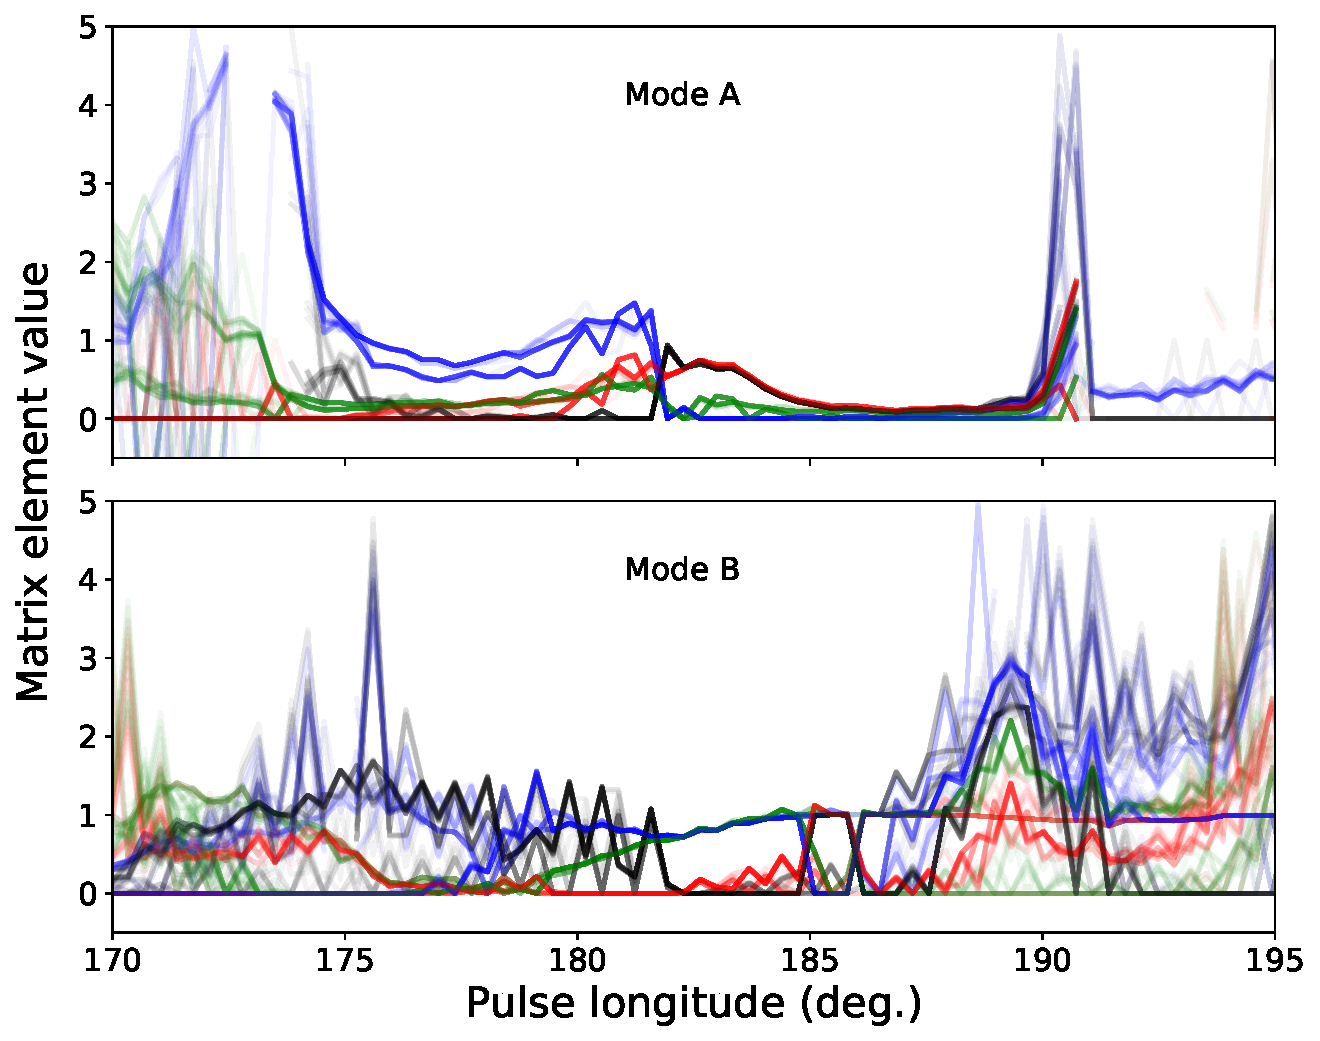
\includegraphics[width=0.8\textwidth]{Figures/B0031/atlas/atlas_matrices}
        \caption[The mixing matrices for the atlas of parameters]{The elements of the mixing matrices produced for the atlas of parameters as a function of pulse longitude. Mode A is shown in the upper panel, and mode B is in the lower panel. The four matrix elements in each are indicated by the coloured lines: $M_{11}$ is red, $M_{12}$ is green, $M_{21}$ is blue, $M_{22}$ is black. The curves appear more opaque where they overlap. As for the matrices shown in Fig.~\ref{fig: B0031 - canonical model driftbands and matrices}, interpolated values are shown for longitudes affected by poor fitting to better show the structure.}
        \label{fig: B0031 - atlas matrices}      
    \end{center}
\end{figure}

In Fig.~\ref{fig: B0031 - atlas matrices} the fitted mixing matrix elements are shown for the 64 solutions for each drift mode to show common features that are independent of the parameter choice. Mode A is shown in the upper panel and mode B in the lower. The range of pulse longitudes shown is limited to $170\degr$ to $195\degr$, as this is corresponds to the region where the results are most stable (i.e. the matrices have generally small values and a clear trend is visible in neighbouring bins).

In both panels the matrix elements appear to be quite robust. In mode A (upper panel) the matrix elements generally vary quite smoothly between pulse longitudes in the on-pulse region, apart from a sharp transition at the fiducial plane. This was expected, given that at this longitude the PA transition is observed to occur in the $P_3$-fold (Fig.~\ref{fig: B0031 - observed P3folds}). At the leading edge of the window, some negative matrix values are still visible -- this is because of floating point precision errors which occur during matrix inversion computation, which especially affects extreme solutions obtained where the observed signal is very weak (and therefore can be neglected). In mode B (lower panel), the mixing matrix in neighbouring longitudes is broadly correlated, and lacks the distinct flip at the fiducial plane seen in mode A. However some variability is visible, especially in the black line (component $M_{22}$) which has a jagged structure such as was observed for the canonical model.

Although the different choices of geometry parameters in the atlas were intended to sample a broad swathe of different potential carousel structures, as for the fitted mixing matrices there are consistent features across the results. To reduce the number of figures in Appendix~\ref{app: atlas results}, results with alias orders $n=5$ and $n=10$ have been omitted, as these higher alias orders are not found to significantly affect the results.

For drift mode A (Figs.~\ref{fig: atlas - MASTER}--\ref{fig: atlas - A_517060014001}), a recurring feature is that at least one of the intrinsic driftbands is V-shaped, meaning that the sub-beams that give rise to this are swept forwards in the azimuthal direction in the carousel frame. This occurs most significantly in OPM 2 (the lower row of panels in each figure), however for some atlas entries the ends of the OPM 1 driftbands (furthest from the fiducial plane) also appear slightly swept forwards. For some geometries there appears to be a small discontinuity in the OPM 1 driftbands on both sides of the fiducial plane, around pulse longitudes $173\degr$ and $191\degr$. Although unclear in the $P_3$-fold, in the magnified sub-beam plot this discontinuity separates two radii of the carousel where the sub-beams appear slightly offset in the azimuthal direction. In some results, for example Fig.~\ref{fig: atlas - A_517005014000}, the discontinuity is present in OPM 2 as well. The sub-beam structure is smooth apart from the discontinuity. This is unlikely to be a `real' structure, in that the boundary appears too sharp to be attributed to nested carousels. It is possible the discontinuity seen in OPM 1 is structure from the more complex driftband shapes of OPM 2 `leaking' into OPM 1. As detailed in Sec.~\ref{sec: B0031 - methods - calculating intrinsic emission - degeneracies}, switching the order of the OPMs is a degeneracy in the solutions. Especially when at least one of the OPMs displays a complex morphology, the algorithm that tries to resolve the degeneracy by forcing smooth structures to be formed might not always succeed.

For mode B the structures seen in the intrinsic driftbands are more diverse. The driftbands as a whole trace the contours of constant $\Theta$ (cyan lines in the $P_3$-folds) without the V-shape that was indicative of strongly swept sub-beams in mode A. Significantly more discontinuities are present in mode B: for example, in Fig.~\ref{fig: atlas - B_517005005000} there is a very sharp jump in the location of the intrinsic OPM 1 driftband at approximately $179\degr$ and $185\degr$, with the portion between these longitudes being offset in $P_3$-fold phase. A similar transition is visible in OPM 2, although this is less abrupt. As shown by the right-hand panels, these transitions are produced by beamlets that are radially extended and vary sharply in azimuth along their length.

Discontinuities of this form are present in nearly all intrinsic driftbands across the atlas for mode B, and as with mode A there appears to be no systematic evolution with the geometry parameters. A recurring feature seen in the magnified sub-beams is that the OPM 2 sub-beams have a backwards sweep ($\Theta$ decreases with increasing $R$) in mode B, whereas OPM 1 of mode A consistently shows a forwards sweep  ($\Theta$ increasing with $R$). From a physical perspective it might be expected that the same sense of sweep is seen in both modes, so this is unexpected -- however, it should be stressed that because each mode was analysed independently they shouldn't be directly compared. This aspect is discussed further in Sec.~\ref{sec: B0031 - discuss - atlas}.

In both drift modes the observed OPMs are recovered well across the atlas, as shown by the middle two plots in each figure in Appendix~\ref{app: atlas results}. For mode A, the change in gradient in the OPM 1 driftband is reproduced, as is the small, faint blob of emission at its leading end. The more compact shape of the OPM 2 driftband is also reproduced well, including its almost rectangular appearance. Similarly, in mode B, the process is clearly successful in reproducing the complex chequerboard pattern at the leading edge of OPM 1 and simultaneously the smooth, continuous bands towards the trailing half (of both OPMs). Compared to the original observed $P_3$-folds (Fig.~\ref{fig: B0031 - observed OPMs}), there appears to be a very small amount of smearing in the $P_3$-fold phase (vertical) direction, the magnitude of which varies stochastically from pulse longitude to pulse longitude. This is most visible in mode A with its higher resolution (due to this mode's greater $P_3$). Some smearing can be expected because the $P_3$-folds of the intrinsic OPMs were forced to be symmetric by averaging data from both sides of the fiducial plane (see Sec~\ref{sec: B0031 - results - literature}). Therefore, any unmodeled features that lead to slight asymmetries will result in broadening. As was the case for the canonical results, there is some bright excess noise in some bins of the $P_3$-folds due to very poor fitting of the mixing matrix. There does not appear to be any systematic variation of where these bad longitudes occur in the atlas results, except that as expected they are more common at locations where the signal is weaker. These results and their implications will be discussed next.







%%%%%%%%%%%%%%%%%%%%%%%%%%%%%%%%%%%%%%%%%%%%%%%%%%%%%%%%%%%%%%%%%%%%%%%%%%%%%%%%%%%%%%%%%%%%%%%%%
%%%%%%%%%%%%%%%%%%%%%%%%%%%%%%%%%%%%%%%%%%%%%%%%%%%%%%%%%%%%%%%%%%%%%%%%%%%%%%%%%%%%%%%%%%%%%%%%%











\section{Discussion}
\label{sec: B0031 - discussion}

The results shown in Sec.~\ref{sec: B0031 - results} and Appendix~\ref{app: atlas results} demonstrate that we have successfully shown that an axially symmetric carousel of sub-beams circulating around the magnetic axis can give rise to the complex, asymmetric $P_3$-folds and polarisation behaviour as observed for PSR~B0031$-$07, if there are two orthogonal polarisation modes which are allowed to mix as they propagate through the magnetosphere. In the following the performance of the canonical model is discussed, and the origin of its parameters is explained. The results of the atlas of geometry parameters are evaluated qualitatively to highlight common features and the goodness-of-fit across the atlas is discussed. Some possible further constraints on the viewing geometry are explained and applied. Finally, the overall results are discussed in the broader context, linking back to the assumptions on which the model was based.


\subsection{The canonical model}
\label{sec: B0031 - discuss - canonical model}

For the `canonical model', which uses parameters for PRS~B0031$-$07 as suggested in the literature, we find a goodness-of-fit (GOF) $\chi^2_R = 6.6$ for drift mode A, and $\chi^2_R = 2.1$ for mode B. This confirms that despite the simplifying assumptions made in the model, it manages to reproduce most details of the complex structures seen in the polarised $P_3$-folds. Mode A has the more complex observed polarisation structures, with reversals in the PA pattern in the leading half of the profile (see Fig.~\ref{fig: B0031 - observed P3folds}, third panels). Despite this, mode B appears to have a much more complex structure in its observed OPMs, in particular the more pronounced chequerboard-like structures in OPM 1 (Fig.~\ref{fig: B0031 - observed OPMs}). The difference in the GOF is likely to be a consequence of the more irregular and curved driftband shapes of the intrinsic OPMs required to fit the observed emission in mode A -- inspection of the $\chi^2$ values (Eq.~\eqref{eq: chi-squared function for asymmetry matrix}) for each pulse longitude bin showed that the fit for mode A was systematically worse than that for mode B, especially closer to the fiducial plane. This potentially means that finer tuning of the geometry parameters is needed or that some assumptions should be relaxed to obtain better fits.

%It is not immediately clear why the GOF is lower for mode B compared to mode A, when from the observed OPMs (Fig.~\ref{fig: B0031 - observed OPMs}) it appears more complex in structure. An onpulse region where the driftbands can clearly be identified is defined for each mode, and the GOF is evaluated over this. Mode A has a smaller on-pulse region by a factor of $\sim$1.4 -- this however should not affect the reduced-$\chi^2$, and does not account for the difference, however a single `bad' fit will carry more weight in this smaller onpulse region. Furthermore, in terms of their shape the mode A driftbands are far more irregular from pulse longitude to pulse longitude, appearing almost rectangular over their short span. This potentially means that finer tuning of the geometry parameters is needed or that some assumptions should be relaxed to obtain better fits.

It should be stressed that during fitting all elements of the mixing matrix were forced to be positive (see Sec.~\ref{sec: B0031 - methods - calculating intrinsic emission} and Appendix~\ref{app: matrix maths - physical constraints}). This physical requirement precludes some possible mathematical solutions that might otherwise fit the data better. So this, alongside other constraints within the model, does not guarantee that good solutions exist for any arbitrary $P_3$-fold. Hence it is highly encouraging that the model produces a good fit. The model was shown to be able to reproduce the data by taking geometrical parameters from the literature, so without any fine-tuning required. As demonstrated by the lower colour plots of Fig.~\ref{fig: B0031 - canonical model driftbands and matrices} which depict the `recovered' observed OPMs arising from a symmetric carousel structure, the observed complexity in the driftbands have been reproduced well. There is slight smearing in the vertical direction which is argued to point towards some asymmetries not being fully reproducible by the model. All main asymmetric features of the observed OPMs shown in Fig.~\ref{fig: B0031 - observed OPMs} have been successfully recovered: these include the small blob on the leading side of mode A, OPM 1, and the chequerboard pattern of OPM 1 of mode B. 

A feature of note is the continuity of the driftbands as seen for the intrinsic OPMs (upper panels in Fig.~\ref{fig: B0031 - canonical model driftbands and matrices}), and the simultaneous continuity of the mixing matrix elements. The continuity of the driftbands was a requirement of the method, achieved by swapping the intensities at a given pulse longitude between the two OPMs if that helps (this is a degeneracy in the model as discussed in Sec.~\ref{sec: B0031 - methods - calculating intrinsic emission - degeneracies}). Swapping of these intensities also necessitates swapping the elements in the columns of the mixing matrix (see Eq.~\eqref{eq: definition of the mixing matrix}). So the elements of the mixing matrix as a function of pulse longitude are not \textit{forced} to be smooth -- nevertheless, this is the case in general. This is what one expects on physical grounds from a magnetosphere with continuous plasma properties and given that the $P_3$-folds are well resolved (without any discontinuities in the observed mode-separated OPMs shown in Fig.~\ref{fig: B0031 - observed OPMs}).

It should be noted that discontinuities in the PA data (for example the OPM transitions visible around the fiducial plane in drift mode A, Fig.~\ref{fig: B0031 - observed P3folds}) do not require a discontinuity in the mode-separated OPMs, nor the mixing matrix. Only a small change in the relative intensities of the OPMs is necessary to produce an OPM transition. However, discontinuities in the observed OPMs do require structure at the corresponding pulse longitude in the mixing matrix. This is further discussed in Sec.~\ref{sec: B0031 - discuss - general discusison}.

% as the figure shows the final matrices are generally smooth. For this dataset with 1024 pulse longitude bins per period, a single longitude bin corresponds to an angle of $0.35\degr$ of stellar rotation. Even taking a low altitude for mixing to occur of 1000~km, this means anisotropies in the magnetosphere would have vary over distances smaller than around 6~km across in order for differences in the mixing matrix to be resolved between longitudes. This is a reasonably large limit, and variations in the magnetosphere can easily occur on smaller scales: for reference, the footprint of the polar cap where the sparks of emission occur has a diameter of $D_\mathrm{PC} \approx 2R\sqrt{R/R_\mathrm{LC}} \approx~300$~m, where $R = 10$~km is the canonical neutron star radius  and $R_\mathrm{LC} = cP/2\pi \simeq  45\times10^{3}$~km  is the light cylinder radius \citep[e.g.][where $c$ is the speed of light]{Sxxx1971}. The observed driftbands are smooth in total intensity which suggests that the magnitude of the variations must intrinsically be small at the altitudes at which mixing may occur.

% Therefore, bin-to-bin variations in the mixing matrix could be expected from both a theoretical (size of the anisotropies) and methodological (forced swapping of neighbouring longitudes) perspective. This could explain the jaggedness of the mode B mixing matrix compared to mode A -- the observed OPMs have a more complex shape (chequerboard pattern), which may be linked to a more turbulent magnetosphere, and hence a greater longitude-to-longitude variation in the mixing matrix would be expected.





\subsubsection{The literature parameter values}
\label{sec: B0031 - discuss - canonical model - literature values}

To create the canonical model we used previously published values of $\alpha$, the number of sub-beams $N$, and the alias order $n$. Here the derivation of these values is discussed, and some of the assumptions that were made.

The value for the magnetic inclination angle came from \citet{SMS+2007}. The authors performed observations of PSR~B0031$-$07 spanning seven different frequency ranges between 150~MHz and 4.85~GHz, using the Giant Metrewave Radio Telescope (GMRT), Westerbork Synthesis Radio Telescope (WSRT), and Effelsberg telescope. They tried three different emission models to model the frequency dependence of the total intensity profile, in order to find a model that reproduced all the features they observed, including the PA curve variations with pulse longitude. Models based on plasma frequency emission and curvature radiation could not reproduce the observations, but an empirical relationship between frequency and emission height that included an extra parameter \citep{Txxx1991} performed well. \citet{SMS+2007} found that RVM models with $\alpha$ between $0.1\degr$ and $6\degr$ were able to reproduce the time-averaged PA curves at different frequencies. We note that because the curvature of the observed PA curve is very low, we find that $\alpha$ and $\beta$ are ill-constrained and highly correlated. However, with a relatively small $\alpha$ \citet{SMS+2007} were able to explain the frequency dependence of the profile width, and the spacing of the subpulses ($P_2$), independent of the polarisation information. Therefore $\alpha = 5\degr$ was considered an appropriate and justifiable value for the canonical model. More detail on the argument that PSR~B0031$-$07 might be a more aligned rotator based on its profile width can be found in Sec.~\ref{sec: B0031 - discuss - atlas - beta constraint}.


% \todo{The viewing geometry was constrained from an initial fit of the RVM, and they found that a range of values between $0.1\degr$ and $6\degr$ was able to reproduce the PA curves at different frequencies.

% \citet{SMS+2007} focused on RVM fitting of data averaged over many pulses, so they would not have observed the intensity modulated OPM changes observed by \citet{IWJ+2020}. They recognised the presence of OPMs and took these into account in their fitting process. Fitting the RVM was also attempted in this work using the single pulse data to better resolve the OPM transitions, but it did not lead to useful constraints since the curvature of the observed PA curve is very low, and thus the $\alpha$ and $\beta$ found using this method are tenuous. Nevertheless, a low $\alpha$ was also found by \citet{SMS+2007} to be able to explain the frequency dependence of the profile width, and the spacing of the sub-pulses ($P_2$), independent of the polarisation information. Therefore $\alpha = 5\degr$ was considered an appropriate and justifiable start point.}

% Forward reference to \ref{sec: B0031 - discuss - atlas - beta constraint}

The values used for the number of sub-beams in the carousel of each mode and their alias orders are those published by \citet{MBW+2019}. The authors take a different approach to \citet{SMS+2007} when examining the drifting subpulses of this pulsar, focusing instead on the periodicities in the pulse stack. They argue that a constant carousel circulation period $P_4$ for all three drift modes is more consistent with the original model of \citet{RSxx1975}, as the speed is determined by the magnetic and electric fields near the surface of the star where the sparks that feed the beamlets occur. These fields cannot easily change their magnitude and/or directions on the timescales at which mode changes can occur (less than one pulse period). Under this assumption, to explain the difference in $P_3$ for each drift mode ($P_3^{(A)} \approx 13P_1$, $P_3^{(B)} \approx 7P_1$, $P_3^{(C)} \approx 5P_1$), \citet{MBW+2019} instead investigate whether a change in the number of beamlets can be responsible. The requirement that $\Delta N$ be an integer immediately means that the alias order cannot be zero for all three drift modes. They argue that if the alias order is the same for all three, then $1/P_3$ is an arithmetic sequence, with the n\textsuperscript{th} term corresponding to a carousel with $N$ sub-beams. If $N_A$, $N_B$, and $N_C$ are in turn themselves part of a sequence, then the values of $P_3$ will be harmonically related (as suggested by \citealt{WFxx1981}), and this can be shown to be the case for PSR~B0031$-$07.
In the special case that the number of beamlets changes by only one between the different drift modes, \citet{MBW+2019} showed that $N_A = 15$, $N_B = 14$, and $N_C = 13$ is a self-consistent solution. This suggests that $n=1$, giving $P_4 \eqsim 16.4 P_1$. Although the \citet{RSxx1975} model predicts a smaller $P_4 \approx 4$, they argue that this solution is much closer to the theoretical value than an unaliased solution. The \citet{RSxx1975} model is well known to predict relatively short circulation periods, and screening of the electric field could be responsible for the difference (e.g. \citet{Sxxx2013} -- it should be noted that this may conflict with the prior assumption of \citet{MBW+2019} that $P_4$ be the same for all drift modes, as the plasma distribution (and hence screening) could differ between modes).

There is a conflict between \citet{SMS+2007} and \citet{MBW+2019}. \citet{SMS+2007} assume that the drifting subpulses are not aliased, and derive the rotation time and number of carousel sub-beams directly from the observed $P_3$ values. They fix the number of sub-beams at $N=9$ for each drift mode, meaning that $P_4$ must change. On the other hand, \citet{MBW+2019} make no comment on $\alpha$ or $\beta$ but do allow aliasing to take place. Therefore, the values used for the canonical model are not fully compatible with all the discussed models. However, since the \citet{MBW+2019} results do not rely on a particular $\alpha$ or $\beta$, the parameters of the canonical model are fully consistent with the \citet{MBW+2019} model. Moreover, there are significant uncertainties associated with each of the parameters used -- this further suggests that the model does not require fine tuning in order to reproduce the observed polarised drifting subpulse patterns.

%%%%%%%%%%%%%%%%%%%%%%%%%%%%%%%%%%%%%%%%%%%%%%%%%%%%%%%%%%%%%%%%%%%%%%%%%%%%%%%%%%%%%%%%%%%%%%%%%
%%%%%%%%%%%%%%%%%%%%%%%%%%%%%%%%%%%%%%%%%%%%%%%%%%%%%%%%%%%%%%%%%%%%%%%%%%%%%%%%%%%%%%%%%%%%%%%%%




\subsection{Atlas of geometry parameters}
\label{sec: B0031 - discuss - atlas}

The atlas of parameters provides a robust examination of the effect of how the choice of the geometry parameters affects the results, and serves to reinforce the findings of the canonical model.

\subsubsection{Goodness-of-fit in the atlas}
\label{sec: B0031 - discuss - atlas - chi2}

As explained in Sec.~\ref{sec: B0031 - results - atlas}, there does not appear to be any systematic variation of the appearance of the results across the entries of the atlas: this is also the case for the goodness-of-fit for each entry. The distribution of reduced-$\chi^2$ values is shown in Fig.~\ref{fig: B0031 - atlas chi2}, where the results for mode A are shown in red and mode B is shown in blue. For mode A, the reduced-$\chi^2$ values are clustered between $4.5$ and $6$, distinctly smaller than the value of $6.6$ obtained for the canonical model. This is not unexpected, since for the canonical model the driftband gradient was forced by a choice of $\beta$ (chosen by fitting the driftband gradient of mode B), whereas in the atlas it is optimised for each entry. The values for mode B are all grouped around the canonical model value of $2.1$, indicating that the specific parameter choice for the canonical model does not perform significantly better than any other. 
\begin{figure}
    \begin{center}
        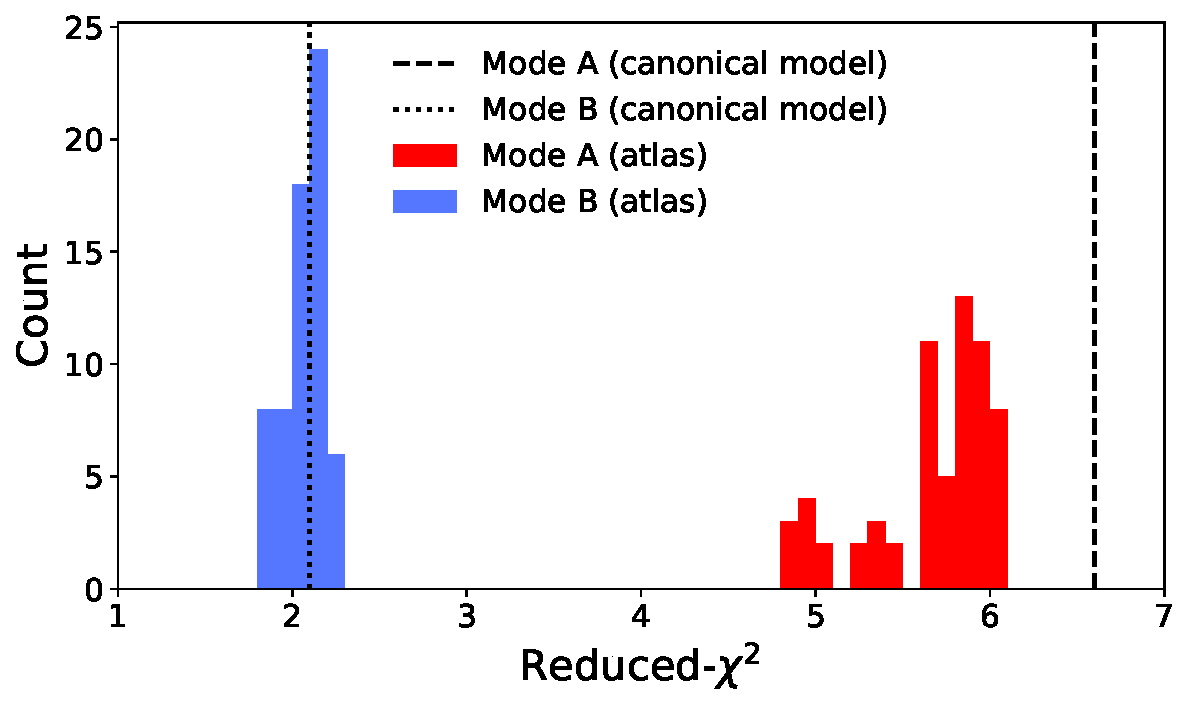
\includegraphics[width=0.75\textwidth]{Figures/B0031/atlas_chi2_hist}
        \caption[Distribution of the goodness-of-fit of the atlas results]{A pair of histograms showing the distribution of reduced-$\chi^2$ values across the 128 atlas entries for drift mode A (red) and mode B (blue). The values for the canonical model parameters for each mode are shown by the dashed and dotted lines respectively.}
        \label{fig: B0031 - atlas chi2}
    \end{center}
\end{figure}
In both modes the reduced-$\chi^2$ is consistently greater than one, without a discernable systematic dependence on the parameter choice. %This was expected to some degree by the degeneracies in the geometry highlighted in Sec.~\ref{sec: B0031 - methods - calculating intrinsic emission} which mean that a reasonable solution can always be found if the driftband gradient is allowed to vary. The clustering of the distributions around the goodness-of-fit found for the canonical model shows that this result is robust.

These results show that the model is robust in the sense that it is insensitive to the geometry parameters that must be assumed. Although the robustness of the mixing model leads to the qualitative conclusion that it can successfully explain the observed asymmetries with an underlying axisymmetric carousel, it also highlights that it is unsuccessful in obtaining meaningful constraints on the required geometry parameters. This may not be surprising given that the duty cycle of PSR~B0031$-$07 over which emission is observable is somewhat limited. This leads to degeneracies between parameters, similar to the process of fitting the RVM to polarisation data (see for example Sec.~\ref{sec: J1926 - analysis - polarisation}). Although more sensitive observations could potentially help for this pulsar, the benefit will be limited.


% This result serves to show that applying the mixing model only leads to qualitative solutions about whether or not a carousel is the source of emission, and it cannot be used to actually quantify the parameters that describe it with precision. Attempting to minimise the reduced-$\chi^2$ of the fit to do so would be fruitless because of the noise in the data which means that underlying systematics cannot be identified -- using data with a higher signal-to-noise ration may lead to a way to constrain the geometry, although the degeneracy of the parameters still remains. The number of assumptions incorporated into our model, from the nature of the carousel emission to the mode separation methods in particular, meant that it was only ever expected to work to first order. Despite this, we have shown that the mixing of the intrinsic modes required to reproduce the asymmetric observations is robust, and independent of the specific geometry of PSR~B0031$-$07

\subsubsection{The fitted mixing matrices}
\label{sec: B0031 - discuss - atlas - mixing matrix}

Figure~\ref{fig: B0031 - atlas matrices} demonstrates that we find a consistent evolution of the mixing matrix elements with pulse longitude over the high S/N on-pulse region, regardless of the choice of geometry parameters for a given drift mode. Although the atlas results suggest that the geometrical parameters related to the carousel structure cannot be constrained by the mode, the required mixing as quantified by the asymmetry matrix \textit{is} constrained. Here it should be noted that the mixing of the OPMs should take place high in the magnetosphere, far from the polar cap where the carousel structure is produced by `sparks' close to the surface of the pulsar (Sec.~\ref{sec: B0031 - introduction}).

While the matrix is similar for all atlas entries of a given drift mode, there is a clear difference in its structure \textit{between} the two modes as shown by the difference between the two panels of Fig.~\ref{fig: B0031 - atlas matrices}. This was not unexpected -- if the magnetosphere must reconfigure to give rise to the significantly different carousel and polarisation properties during mode switching, there is no reason why the magnetospheric mixing and attenuation during propagation would not be affected. As such, this means that mode switching should be considered to be a \textit{global} magnetospheric phenomenon rather than something that only affects the polar cap area. This is not a new idea: for example, nulling (see Chapter~\ref{chapt: J1926} for instance) is thought to be an extreme form of mode change \citep[e.g.][]{Bxxx1992,WMJx2007} caused by the global reconfiguration of magnetospheric currents \citep{KLO+2006,Txxx2010b}. 

The mode changes in PSR~B1957+20 that affect multiple components in both the main and interpulse profiles \citep{MKMP2018} also provide evidence for large-scale magnetospheric changes. \citet{WWJx2012} noted that PSR~B1055$-$52, which is a nearly orthogonal rotator, exhibits phase-locked modulation in the emission from both its magnetic poles. A comparable behaviour was observed in PSR~B1702$-$19, which has periodic modulation with $P_3 \sim 11P_1$ in both its main pulse and interpulse profiles, with a phase lag of approximately half a stellar rotation \citep{WWSx2007}. A third example of global magnetospheric changes are found for another interpulse pulsar, PSR~B1822$-$09 \citep{BMRx2010}. This object displays mode-switching behaviour, with distinct `bright' (B) and `quiescent' (Q) states \citep{FWMx1981}. In the B-mode, the main pulse gains an additional profile component whilst the interpulse emission vanishes -- the intensities of the radiation produced by the two poles are anti-correlated \citep{FWxx1982, GJKx1994}. This persists in the Q-mode, to a lesser extent \citep[Fig. 11]{BMRx2010}. Overall, these objects provide strong evidence that emission is influenced by global magnetospheric behaviours, which might well apply to PSR~B0031$-$07 as well.


\subsubsection{Evaluation of the atlas plots}
\label{sec: B0031 - discuss - atlas - atlas plots evaluation}

To reiterate the point raised in Sec.~\ref{sec: B0031 - methods - calculating intrinsic emission - degeneracies}, the intrinsic OPMs shown ($P_3$-folds and carousels such as in Fig.~\ref{fig: B0031 - canonical model sparks and carousels}) are not unique solutions, nor are the mixing matrices. The intrinsic OPMs shown in Appendix~\ref{app: atlas results} may still be a linear combination of X- and O-mode emission, as the mixing matrices shown in Fig.~\ref{fig: B0031 - atlas matrices} are only one possible solution to the degeneracy, as explained in Sec.~\ref{sec: B0031 - methods - calculating intrinsic emission - degeneracies}. That said, the atlas of results can provide some insight into the required carousel structure when the entries share common features. 

In the atlas, we found that for mode A one intrinsic OPM (usually OPM 2) exhibited V-shaped driftbands whereas the other largely traced the contours of constant $\Theta$. This is a consequence of the beamlets being swept azimuthally in the carousel, and the non-swept beamlets are more compact. This could be related to refraction effects, as introduced in Sec.~\ref{sec: B0031 - introduction}. \citet{BAxx1986} associated the two OPMs with the O- and X-mode propagation of radiation in a strongly magnetised, ultra-relativistic plasma. The X-mode experiences no refraction whereas the O-mode does, and therefore is slightly delayed in pulse longitude. The swept-out sub-beams of OPM 2 could be a signature of refraction that distorts initially compact beamlets, such as seen in OPM 1. We assigned the labels OPM 1 and OPM 2 arbitrarily so they are not necessarily associated with a specific plasma mode; nevertheless, the consistency of the sub-beam shape across the mode A atlas means that the patterns labelled OPM 1 and 2 may be dominated by X- and O-mode emission respectively.

The mode B results show much more variability across the atlas, with much more complex driftband shapes. As explained in Sec.~\ref{sec: B0031 - results - atlas} there are some entries which show a sweep in the beamlets for one or both of the OPMs, but nowhere near as consistently as in mode A. The more common feature is a discontinuity in the driftband which originates from two concentric rings of beamlets, offset azimuthally in the carousel frame. The amount of offset varies, as does the sharpness of the transition. These discontinuities are likely caused by confusion of the smoothing algorithm rather than any real feature in the intrinsic driftbands, which are otherwise smooth. As explained in Sec.~\ref{sec: B0031 - methods - calculating intrinsic emission - degeneracies}, one of the steps taken in producing the intrinsic driftbands is to swap intensities between the two OPMs in order to make the driftbands as continuous as possible. This process begins at the fiducial plane and moves outward, and two sets of longitudes in the leading and trailing halves are compared simultaneously with the neighbouring (inner) longitudes. Initially (close to the fiducial plane) the driftbands of mode B are very smooth and have a high S/N so this process is reliable and will always lead to smooth results. However, around $177\degr$ pulse longitude OPM 2 becomes significantly weaker (see Fig.~\ref{fig: B0031 - observed OPMs}), corresponding to the location of the discontinuity in the intrinsic OPM. The smoothing algorithm was likely confused by the noisy pulse longitude bins in the intrinsic OPMs caused by poor fitting to the weak signal in the observed OPM 2, coupled with the transition to the chequerboard-like pattern in OPM 1.

Clearly the observed mode B is much more complex than mode A in terms of the separated observed OPMs (Fig.~\ref{fig: B0031 - observed OPMs}), but arguably also in total intensity (Fig.~\ref{fig: B0031 - observed P3folds}, top panels). The question is, from where should the complexity originate? The carousel of sparks should arguably be relatively simple in structure if it is to be maintained during circulation in the polar cap. That would favour beamlets that are compact as seen for example in PSR~B0809+74 \citep{RRL+2006}, but note also that one OPM on this carousel (their Fig.~10) has swept sub-beams as we found in mode A of PSR~B0031$-$07. Our method of determining the mixing matrix from the fitted asymmetry matrix (Appendix~\ref{app: matrix maths - posmatrix explanation}) attempts to force as much of the complexity into the mixing matrix (i.e. magnetospheric processes) and have the carousel be as simple as possible. The discontinuities in the fitted intrinsic driftbands of mode B suggests that some complexity still remains in the intensity rather than the mixing matrix. Here it should be stressed that the intrinsic beam patterns derived may have been affected by refractive processes in the magnetosphere (see Sec.~\ref{sec: B0031 - methods - magnetospheric distortions}), which will add complexity on top of the pattern of sub-beams produced in the polar cap.


\subsubsection{Further constraints on the geometry}
\label{sec: B0031 - discuss - atlas - beta constraint}

A further constraint on the results to be considered comes from the values of the impact parameter $\beta$ in the atlas. In order for emission to be observed, the observer's line of sight must intersect the emission cone surrounding the magnetic axis. The relationship between the observed profile width $W$ (assuming the emission fills the open-field-line region), the geometry of the LOS as quantified by $\alpha$ and $\beta$, and the half opening angle of the emission cone $\rho$ is
\begin{equation}
    \label{eq: B0031 - allowed geometry}
    \cos\rho = \cos\alpha\cos(\alpha+\beta)+\sin\alpha\sin(\alpha+\beta)\cos\bigg(\frac{W}{2}\bigg),
\end{equation}
as derived by \citet{GGRx1984}, and see also Appendix~\ref{app: geometry derivations}. For the LOS to intersect the cone, $\rho \geq |\beta|$. In our method $\beta$ was not an input into the model directly, but rather was derived from the best-fitting driftband gradient in combination with the other parameters (see Sec.~\ref{sec: B0031 - methods - parameter space}). Figure~\ref{fig: B0031 - atlas alpha vs beta} shows the derived values for the LOS colatitude $\alpha + \beta$ corresponding to the different values of $\alpha$ -- results for mode A are shown in red, and for mode B they are blue.
\begin{figure}
    \begin{center}
        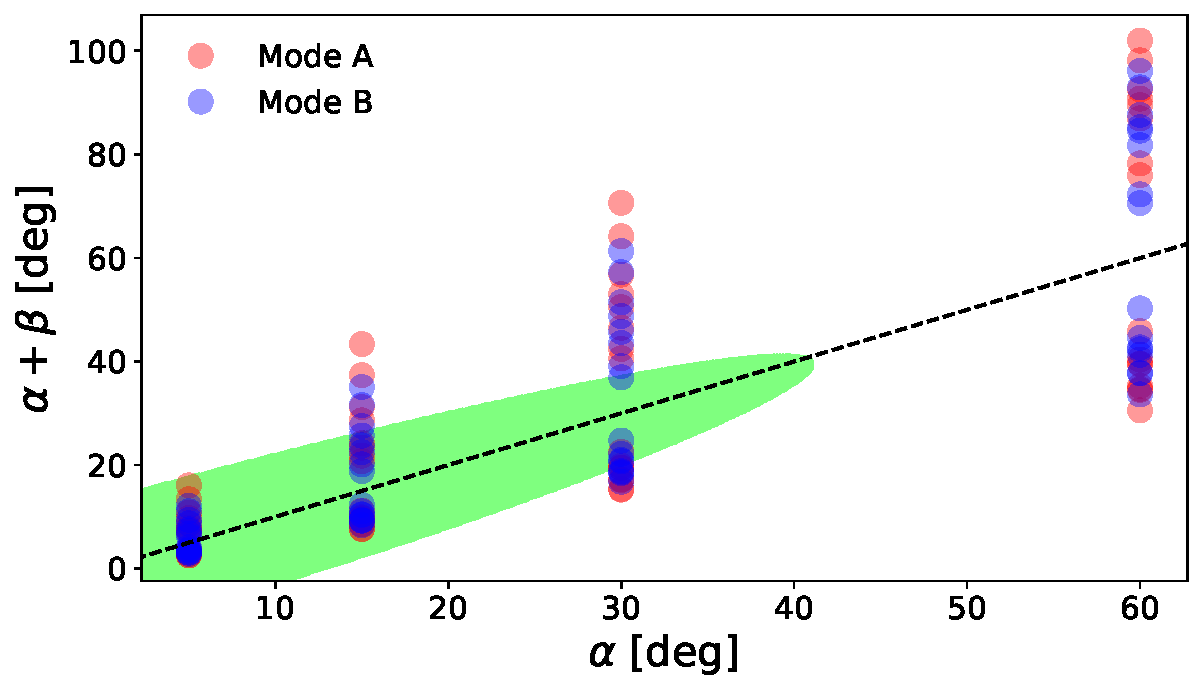
\includegraphics[width=0.75\textwidth]{Figures/B0031/alpha_zeta_distribution}
        \caption[Distribution of $\alpha$ and $\beta$ in the atlas of results]{The colatitude of the LOS $\alpha + \beta$ plotted against the magnetic inclination angle $\alpha$ for the atlas of results. Mode A is shown in red, and mode B is shown in blue. Mode A permits slightly larger values of $|\beta|$ than mode B due to larger driftband gradient, $m$. The dashed black line indicates $\beta = 0$. The green region indicates which values of $\alpha$ and $\beta$ satisfy Eq.~\eqref{eq: B0031 - allowed geometry} for a profile width of $W = 40\degr$ and emission cone half opening angle $\rho = 13\degr$.}
        \label{fig: B0031 - atlas alpha vs beta}     
    \end{center}
\end{figure}
The sign of $\beta$ depends on the alias order, as seen in Eq.~\eqref{eq: driftband gradient}. This is because the apparent drift direction depends on the alias order, and it also depends on whether the carousel is viewed by an inner or outer line of sight. The observed driftbands have a negative gradient, and this is predicted if $\beta < 0$ for even alias orders, and $\beta > 0$ for odd alias orders as shown in Appendix~\ref{app: geometry derivations}. %A hard geometry requirement is that $0\degr \leq \alpha + \beta < 180\degr$ and all values in Fig.~\ref{fig: B0031 - atlas alpha vs beta} satisfy this. If any atlas entry had broken this constraint this would have provided a way to rule out that choice of the other geometry parameters ($N$, $n$, and $\alpha$). 

In both modes in the atlas, $\beta$ is in general permitted to be quite large, especially for large values of $\alpha$: this would require very large emission cones. The opening angle of the emission cone is governed by the tangents to the last open field lines at the emission height, so a large cone in turn requires exceptionally large altitudes. Given PSR~B0031$-$07 is a `normal' pulsar in terms of its spin properties, this seems unlikely \citep[e.g][]{GLxx1998,  WJxx2008, JKxx2019}. 
Assuming an upper bound on the emission height $h_\mathrm{em}$ of 1000~km \citep[e.g.][]{KJxx2007}, the opening angle of the emission cone is given by 
\begin{equation}
    \label{eq: B0031 - cone angle}
    \rho = \sqrt{\frac{9\pi h_\mathrm{em}}{2cP}}
\end{equation}
in the small angle limit \citep[e.g. $h_\mathrm{em} \ll R_\mathrm{LC}$,][]{Rxxx1990}. This gives $\rho \approx 13\degr$. The profile width of PSR~B0031$-$07 $W \approx 40\degr$. Substituting these values into Eq.~\eqref{eq: B0031 - allowed geometry} provides a way to constrain values of $\alpha$ and $\beta$ which satisfy the relation. These `allowed geometries' are shown as the green region in Fig.~\ref{fig: B0031 - atlas alpha vs beta}, and indicate that $\alpha \lesssim 40\degr$. This provides an argument that lower values of $\alpha$ are desirable, in agreement with the modelling of \citet{SMS+2007} which was based on the observed profile width and frequency dependence of $P_2$. In this it should be noted that we only considered a relatively small sample of values for $N$ and $n$ in our atlas, which also contribute to $\beta$ for a given $\alpha$ and measured driftband gradient $m$ (Eq.~\eqref{eq: driftband gradient}). However, the sample covers a wide range of possible parameter space. The dependence of $|\beta|$ on these two parameters is only a small, positive correlation, so does not greatly affect our overall conclusions.





%%%%%%%%%%%%%%%%%%%%%%%%%%%%%%%%%%%%%%%%%%%%%%%%%%%%%%%%%%%%%%%%%%%%%%%%%%%%%%%%%%%%%%%%%%%%%%%%%
%%%%%%%%%%%%%%%%%%%%%%%%%%%%%%%%%%%%%%%%%%%%%%%%%%%%%%%%%%%%%%%%%%%%%%%%%%%%%%%%%%%%%%%%%%%%%%%%%








\subsection{General discussion}
\label{sec: B0031 - discuss - general discusison}

A key assumption in this work is that coupling of the OPMs can occur in the pulsar, at altitudes higher than those at which refraction is the dominant magnetospheric effect on polarisation. This has been suggested in the literature, but is at some level a simplification as refraction and mode coupling are closely related phenomena. For example, \citet{Pxxx2001} argues that refraction is significant only at distances of the order of the emission altitude since the plasma number density rapidly decreases with altitude ($\rho \propto r^{-3}$; e.g. \citealt{RSxx1975}).
At the altitudes at which emission is produced, the two modes do not interact with each other and their polarisation evolution can be described in terms of geometrical optics -- the plasma is sufficiently dense that refraction is a significant effect. At some point during their propagation, the light rays will travel quasi-longitudinally with the local magnetic field lines, at which point geometrical optics fails. In this region of conversion \citet{Pxxx2001} argues that energy can be transferred from the subluminous O- to the superluminous X-mode. Eventually, the rays deviate from the magnetic field once more; mode coupling no longer takes place, and geometrical optics is once again valid. However, the plasma density has fallen by this point such that refraction is no longer significant. The waves propagate independently, although they may acquire some circular polarisation and the PA may rotate slightly until they reach the polarisation limiting region \citep{PLxx2000, Pxxx2001}.


An important step in applying our model was separating the observed polarised emission into two independent OPMs, broadly following the method of \citet{MSxx2000}. The mode separation was built on assumptions which will affect the results if inaccurate. The assumptions made were 1) that the two OPMs are perfectly orthogonal, and 100~per~cent linearly polarised, and 2) that the OPMs combine by incoherent mode addition. As explained in Sec.~\ref{sec: B0031 - methods - mode separation}, we neglected the circularly polarised emission as it is considerably weaker than the linearly polarised emission, so contributes very little to the overall intensity of both Stokes $I$ and the two orthogonal modes. However, the presence of circular polarisation gives rise to strange behaviour in the $P_3$-folds, as noted by \citet{IWJ+2020}. At the PA transition, where the dominant OPM switches, the ellipticity angle is at its maximum, where the expected signature of truly orthogonal emission is that it should be zero. This can possibly be explained if the two OPMs are not perfectly orthogonal, such that the ellipticity angle of one OPM is slightly larger than the other. Then, at a transition, as one OPM decreases in intensity and the other increases, the resultant vector on the Poincar\'e sphere would sweep round in azimuth (PA), but also pass through one of the poles (associated with pure Stokes $V$) in the process. Non-orthogonal polarisation modes may therefore need to be considered in order to more accurately mode-separate the data, but the methods would be much more complex as this would require knowledge about the ellipticity angles of each mode, as well as whether their offset remains constant at all times. Given the small degree of circular polarisation in PSR~B0031$-$07, this will be of little consequence.


One can also consider what effect coherent mode addition may have. In that case it is in principle possible to produce any orientation of a vector in the Poincar\'e sphere by summing the two contributing modes with a suitable intensity ratio and phase offset \citep[e.g.][]{Dxxx2017}. Coherent processes are thought to take place in pulsar magnetospheres; for example it is coherent radio emission from bunches of charged particles which leads to the bright polarised emission in the first place \citep{RSxx1975}. While all radiation is produced coherently on a microscopic scale, radiation originating from macroscopically separated locations in the magnetosphere do not necessarily add coherently, as this depends on the coherence length of the radiation. As for non-orthogonal polarisation modes, attempting to explain the observations as coherent mode addition requires more assumptions on the magnitudes, orientations, and phases of the constituent waves, thereby making the model less constraining. We know that incoherent mode addition must play a role given the significant degree of depolarisation observed for PSR~B0031$-$07. The approach of taking incoherent mode addition as the basis for modelling can therefore be viewed as a first-order approximation. 

Although we have demonstrated that the OPM mixing model could explain complicated pulsars such as PSR~B0031$-$07, the resulting degeneracies in the solutions make it hard to reach any firm conclusions about the behaviour of the pulsar magnetosphere. However, the relative amplitudes of the mixing matrix elements can give some information on the origin of the structures visible in the observed OPMs. For example, consider OPM 2 of drift mode A (lower left panel of Fig.~\ref{fig: B0031 - observed OPMs}): at approximately $182\degr$ there is a slight `kink' in the observed driftband such that there appears to be an offset in phase. In the fitted mixing matrix for both the canonical model (Fig.~\ref{fig: B0031 - canonical model driftbands and matrices}; lower left panel) and the atlas (Fig.~\ref{fig: B0031 - atlas matrices}), element $M_{21}$ (blue line) is strong in the leading half while $M_{22}$ (black line) is close to zero, and vice versa in the trailing half. This shows that the kink in the observed OPM is due to a sudden swap between emission from intrinsic OPM 1 to intrinsic OPM 2. In the framework of \citet{Pxxx2000} this may indicate a transition between a region where mode conversion is a strong effect to one where it is not, caused by the geometry of the underlying magnetic field and/or plasma distribution at the observed pulse longitude. 

% \todo{For example, when pairs of elements switch this tells use where the dominant mode changes. A solution for the mixing matrix which is the same for two drift modes could exist, but not for PSR~B0031$-$07. This can be seen from the observed OPM $P_3$-folds as shown in Fig.~\ref{fig: B0031 - observed OPMs}. Looking at OPM 1 in this Figure (upper $P_3$-fold panels), there is a region between pulse longitudes $170\degr$ to $180\degr$ where mode A has a continuous driftband but mode B is in a transition state. This cannot occur if the mixing matrix were the same in both modes, and serves to illustrate that the state of the magnetosphere must change between modes, in a way that is not just limited to the emission region.}

The chequerboard pattern in the observed leading half of mode B led to the expectation that mode switching is occurring often across this region, and this is borne out in the mixing matrix shown in Fig.~\ref{fig: B0031 - canonical model driftbands and matrices}. On the other hand, the mixing matrix for mode A is much smoother and transitions happen less frequently. The evidence of more complex mixing behaviour for mode B may suggest that the magnetosphere is becoming less homogeneous in this mode. It is not clear whether a change in the carousel morphology triggers the more variable magnetosphere, or vice versa, or indeed if the two are independent but symptoms of some larger underlying change. If extensions to this model are to be explored, then some model of how the mixing depends on the state of the magnetospheric plasma is required. This can then lead to predictions of the mixing matrix from a given carousel state which could then be tested against observations.





%%%%%%%%%%%%%%%%%%%%%%%%%%%%%%%%%%%%%%%%%%%%%%%%%%%%%%%%%%%%%%%%%%%%%%%%%%%%%%%%%%%%%%%%%%%%%%%%%
%%%%%%%%%%%%%%%%%%%%%%%%%%%%%%%%%%%%%%%%%%%%%%%%%%%%%%%%%%%%%%%%%%%%%%%%%%%%%%%%%%%%%%%%%%%%%%%%%








\section{Conclusions}
\label{sec: B0031 - conclusion}


Overall, it has been successfully established that asymmetric driftband patterns in both total intensity and polarisation can be caused by the pulsar magnetosphere distorting the emission from (circular) axisymmetric carousel-like structures. Here the asymmetry is modelled as arising from the (pulse longitude-dependent) mixing and attenuation of two OPMs as they propagate through the magnetosphere. This was parametrised with a `mixing matrix', fitted by comparing the emission observed at pulse longitudes on either side of the fiducial plane $\phi_\mathrm{fid}$ which are produced by the same part of the circulating pattern in the carousel. An `atlas' of possible geometry parameters was investigated, including a `canonical model' which was based on previously published values for the viewing geometry and number of sub-beams in and alias order of the carousel. 

The observations do not provide sufficient information for the method to pin down specific values for any parameter, due to degeneracies. However, the complex and asymmetric $P_3$-folds for each OPM in each drift mode have been robustly reproduced using both the canonical geometry parameters and others. This includes the chequerboard pattern in one of the OPMs in drift mode B. For this drift mode, a diversity of structures were found for the intrinsic pattern of sub-beams corresponding to the OPMs before being distorted by the mixing matrix, which were not systematically dependent on the geometry parameters. However, a common observation for drift mode A is that one intrinsic OPM has azimuthally swept sub-beams whilst for the other mode the sub-beams are more compact; this could be similar to the structure of the sub-beams in the carousel of PSR~B0809+74 when viewed as two OPMs \citep{RRL+2006} and may be due to the refraction of one OPM \citep[The O-mode;][]{ABxx1986} before mixing.

This result demonstrates that applying the mixing model in its present form mainly leads to qualitative results, such as confirming that despite the observed asymmetries a carousel could be the source of emission. The model cannot be used to quantify the parameters that describe it with precision. This is because of degeneracies in the model, and the model itself not fully describing the complexities of pulsar magnetospheres. The number of assumptions incorporated into our model, from the nature of the carousel emission to the mode separation methods in particular, meant that it was never expected to be fully compatible with the data. Despite this, we have shown that the mixing of the intrinsic modes required to reproduce the asymmetric observations is robust, and independent of the specific geometry of PSR~B0031$-$07. The difference between the mixing matrices found for the two drift modes therefore provides further evidence that a global reconfiguration of the magnetosphere is responsible for mode changes in pulsars, as both the polar cap physics and the mixing much higher up in the magnetosphere are affected simultaneously.

For both drift modes it was found that the mixing matrices fitted for each entry in the atlas of results are very similar in structure where the pulsar signal is strong. This result confirms that the required OPM mixing is largely independent of the choice of geometry parameter, and is separable from the geometry parameters determining the carousel structure. The goodness-of-fit (a reasonably low reduced-$\chi^2$) of the results was found to be insensitive to the geometry parameters, and demonstrates that most of the complex features are successfully reproduced. That a similar mixing model is able to fit the observations over a wide range of geometry parameters is perhaps unsurprising, as the carousel emission is produced in the polar cap while the mixing occurs significantly higher in the magnetosphere, so the two processes should be largely independent.

In conclusion, magnetospheric mixing is a natural way to allow drifting subpulses with highly asymmetric (polarised) behaviour to be produced by the widely adopted (axisymmetric) carousel model. Despite the fact that observations of PSR~B0031$-$07 seem at first glance to rule out the carousel model, it in fact remains a viable explanation for the origin of drifting subpulses. The methodology presented here would be much more valuable if the magnetospheric mixing effects could be predicted theoretically, or could at least be linked to the required plasma properties. The model could be applied to the broader population of pulsars which exhibit subpulse drifting -- this could highlight correlations between a pulsar's observed single-pulse behaviour and constraints obtained for magnetospheric mixing. Given that the magnetosphere state is linked to (if not determined by) the carousel structure and circulation, such correlations can be expected.